\newpage
\chapter{Фрактальные квадраты с конечным пересечением}

В данной главе мы рассмотрим частный случай фрактальных $k$-кубов --- фрактальные квадраты.

\begin{definition}\label{dfn:FS} 
Пусть $D=\{d_1,\ldots,d_m\}\IN\{0,1,\ldots,n-1\}^2$, где $n\ge 2$, и $1<m<n^2$.
{\em Фрактальным квадратом} порядка $n$ с {\em множеством единиц $D$} называют компактное множество $K\IN\rr^2$, удовлетворяющее уравнению
$$
K=\dfrac{K+D}{n}.
$$
\end{definition}

\begin{figure}[h]
 \centering
 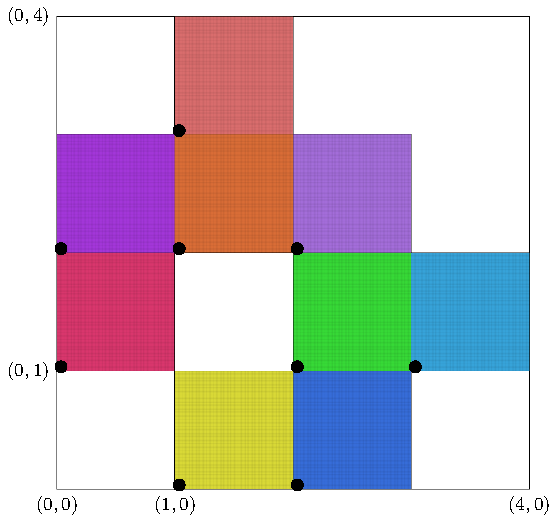
\includegraphics[width=0.48\textwidth]{digitset.pdf}
 \hfill
 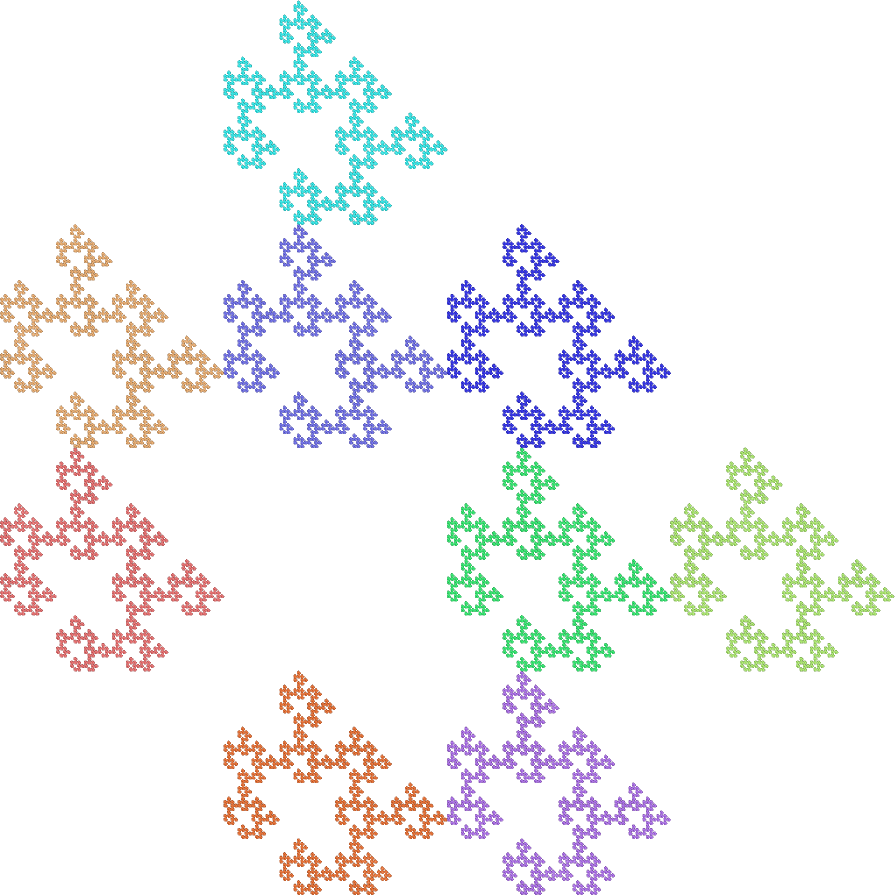
\includegraphics[width=0.42\textwidth]{den2f.png}
 \caption{Множество $n(D+P)$ (слева) и фрактальный квадрат $nK=K+D$ (справа). Элементы из $D$ отмечены чёрными точками.}
 \label{fig:fr_sq}
\end{figure}


\begin{corollary}
Если $\bma\in\{(1,0),\ (-1,0),\ (0,1),\ (0,-1)\}$ и $\#F_\bma>1$, то $F_\bma$ (см. определение \ref{def:F_alpha}) связно тогда и только тогда, когда оно является отрезком.
\end{corollary}

\begin{proof}
Если $F_\bma$ неодноточечно и связно, то множество $K_{\bma}$ содержит неодноточечное связное подмножество, значит, $\dim_H(K_{\bma})\geq1$.
В силу Предложения \ref{prop:Ka}, множество $K_{\bma}$ имеет размерность $\dim_H(K_{\bma})=\log_n\#D_{\bma}$.
Поскольку $\#D_{\bma}\leq n$, неравенство $\dim_H(K_{\bma})\geq1$ возможно только если $\#D_{\bma}= n$.
Такому множеству единиц $D_{\bma}$ соответствует фрактальный квадрат $K_{\bma}$, совпадающий с ребром $P_{\bma}$.
Аналогично, $K_{-\bma}=P_{-\bma}$.
Из этого следует, что $F_\bma=K_{\bma}=P_{\bma}$.
\end{proof}


\subsection{Мощность пересечений копий фрактального квадрата}

%Рассмотрим фрактальный квадрат $K=\dfrac{K+D}{n}$ и пару таких копий $\dfrac{K+d_1}{n}$ и $\dfrac{K+d_2}{n}$, что $d_2=d_1+\bma$, где $\bma\in A\mmm\{0\}$.
%Назовём такую пару копий {\em копиями с $\bma$-соседством}.
%Тогда $\dfrac{K+d_1}{n}\cap\dfrac{K+d_2}{n}=\dfrac{d_1+F_\bma}{n}$, значит мощность пересечения копий с $\bma$-соседством совпадает с мощностью множества $F_\bma$.
Сформулируем следствие из теоремы \ref{fin_int}, позволяющее оценить мощность множества $F_\bma$ при $\bma\in A\mmm\{0\}$ в случае фрактальных квадратов.

\begin{corollary}\label{fin_int_sq}
\qquad
%Пусть $K=\dfrac{K+D}{n}$ --- фрактальный квадрат.
% Рассмотрим $F_\bma, \bma\in A\mmm\{0\}$.
\begin{itemize}[nolistsep]
 \item[(i)] Если $\#G_{\bma}> 1$, то множество $F_\bma$ несчётно.
 \item[(ii)] Если $\#G_{\bma}=1$ и существует $\bmb\sqsupset\bma$ такое, что  $F_\bmb$ непусто и $\#G_{\bma\bmb}\geq1$, то $F_\bma$ счётное.
 \item[(iii)] Множество $F_\bma$ конечно в следующих случаях:
 \begin{itemize}[nolistsep]
 \item[\textbf{(a)}] $\#G_{\bma\bma}=1$ и $\#F_\bmb\cdot\#G_{\bma\bmb}=0$ для каждого $\bmb\sqsupset\bma$;
 \item[\textbf{(b)}] $\#G_{\bma\bma}=0$ и существует $\bmb\sqsupset\bma$ такое, что $\#F_\bmb\cdot\#G_{\bma\bmb}\geq1$.
 \end{itemize}
\end{itemize}\qed 
\end{corollary}

%\begin{proof}
%При $\bma\in A\mmm\{0\}$ множество $F_\bma$ удовлетворяет уравнению
%$F_\bma=\bigcup\limits_{\bmb\sqsupseteq\bma} \dfrac{F_\bmb+G_{\bma\bmb}}{n}$, 
%где $G_{\bma\bmb}=D_\bma\cap(D_{-\bma}+n\bma-\bmb)$.\\
%Если $\bma\in\{(1,0),\ (-1,0),\ (0,1),\ (0,-1)\}$, то $\#\{\bmb:\bmb\sqsupset\bma\}=2$, при этом $\bmb\in\{(1,1),\ (-1,1),\ (1,-1),\ (-1,-1)\}$.\\
%Если $\bma\in\{(1,1),\ (-1,1),\ (1,-1),\ (-1,-1)\}$, то $\#\{\bmb:\bmb\sqsupset\bma\}=0$.\\
%
%Для $\bma\in\{(1,1),\ (-1,1),\ (1,-1),\ (-1,-1)\}$, то $\#G_{\bma\bmb}\leq1$ множество $F_\bma$ не более чем одноточечно.\\
%
%Далее предполагаем, что $\bma\in\{(1,0), (-1,0), (0,1), (0,-1)\}$.\\
%
%(i) Если $\#G_{\bma\bma}> 1$, то $F_\bma$ содержит в себе фрактальный квадрат с множеством единиц $G_{\bma\bma}$, который имеет мощность континуума.\\
%
%(ii) Рассмотрим случай, когда $\#G_{\bma\bma}=1$ и существует $\bmb\sqsupset\bma$ такое, что  $F_\bmb$ непусто и $\#G_{\bma\bmb}\geq1$. 
%Такое непустое $F_\bmb$ единственно, поскольку иначе $\#G_{\bma\bma}>1$.
%Множество $\dfrac{F_\bmb+G_{\bma\bmb}}{n}$ конечно, поэтому $F_\bma=\bigcup\limits_{n=1}^\8 S_\bma^n$.\\
%
%(iii.{\bf a}) Пусть $G_{\bma\bma}=\{d_i\}$ и $\#F_\bmb\cdot\#G_{\bma\bmb}=0$ для каждого $\bmb\sqsupset\bma$.
%В этом случае из равенства $F_\bma=\dfrac{F_\bma+\{d_i\}}{n}$следует $F_\bma=\left\{\dfrac{d_i}{n-1}\right\}$.\\
%
%(iii.{\bf b}) Наконец, рассмотрим случай, когда $G_{\bma\bma}=\0$ и существует $\bmb\sqsupset\bma$ такое, что $\#F_\bmb\cdot\#G_{\bma\bmb}\geq1$.
%При $G_{\bma\bma}=\0$ может существовать не более одного $\bmb\sqsupset\bma$ такого, что $F_\bmb\neq\0$, в противном случае $\#G_{\bma\bma}\geq2$.
%Так как $\#F_\bmb=1$, множество $F_\bma=\dfrac{F_\bmb+G_{\bma\bmb}}{n}$ конечно, а говоря точнее, $\#F_\bma=\#G_{\bma\bmb}$.
%\end{proof}

\begin{corollary}\label{onepoint} 
Если $F_\bma$ конечно, то  $\#F_\bma=\#G_{\bma\bmb}\leq\left\lfloor\dfrac{n-2}{2}\right\rfloor$.
\end{corollary}

\begin{proof}
Если множество $F_\bma$ удовлетворяет условию (iii.{\bf a}) следствия \ref{fin_int}, то оно не более чем одноточечно.

Рассмотрим теперь множество $F_\bma$, удовлетворяющее условию (iii.{\bf b}) следствия \ref{fin_int}.
Не ограничивая общности, положим $\bma=(0,1)$, $\bmb=(-1,1)$ и $F_\bmb\neq\0$.
Значит, $\{(0,n-1),\ (n-1,0)\}\IN D$.
Сразу отметим, что $F_{(-1,-1)}=F_{(1,1)}=\0$, так как в противном случае $\#G_\bma>1$ и $F_\bma$ несчётно.

\begin{figure}[h!]
\centering
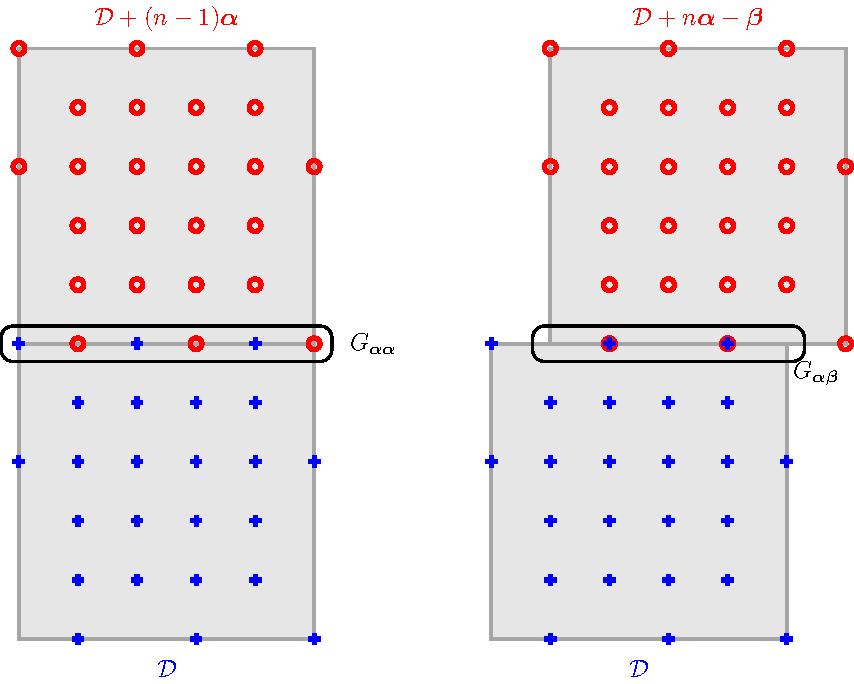
\includegraphics{Gab_card.pdf}
 \caption{Множества $G_{\bma}$ и $G_{\bma\bmb}$ при $\bma=(0,1)$ и $\bmb=(-1,1)$.}
 \label{fig:Gab}
\end{figure} 

Очевидно, что при любом $D$ справедлива оценка $\#G_{\bma\bmb}\leq n-1$, что показано на рисунке \ref{fig:Gab}.
Из $(0,n-1)\notin (D+n\bma-\bmb)=D+(1,n-1)$ следует, что $(0,n-1)\notin G_{\bma\bmb}$.
Если $(n-1,n-1)\in G_{\bma\bmb}$, то $(n-2,0)\in D$, но тогда, согласно Теореме \ref{fin_int}, множество $F_\bma$ бесконечно.
Значит, $(n-1,n-1)\notin G_{\bma\bmb}$.

Из условия (iii.{\bf b}) следует равенство $G_{\bma}=\0$, поэтому для каждого $d\in G_{\bma\bmb}$ справедливы соотношения $(d-n\bma+\bma)\notin D$ и $(d-n\bma+\bmb)\in D$.
Значит, для любого $d\in D$ пара координат вида $\{d,\ d+(1,0)\}$ (или, в общем случае, пара $\{d,\ d+\bma-\bmb\}$) не может содержаться в множестве $G_{\bma\bmb}$.
Учитывая, что $(0,n-1),\ (n-1,n-1)\notin G_{\bma\bmb}$, справедлива оценка 
$$\#G_{\bma\bmb}\leq\left\lfloor\dfrac{n-2}{2}\right\rfloor.$$
\end{proof}

Далее докажем, что фрактальный квадрат, являющийся дендритом, обладает свойством одноточечного пересечения.
Поэтому укажем условия, при которых $F_\bma$ одноточечно:

\begin{corollary}\label{onepoint} 
Множество $F_\bma$ одноточечно, если \\
\textbf{(a)} $\#G_{\bma\bma}=1$ и $\#F_\bmb\cdot\#G_{\bma\bmb}=0$ для каждого $\bmb\sqsupset\bma$; или\\
\textbf{(b)} $\#G_{\bma\bma}=0$ и существует $\bmb\sqsupset\bma$ такое, что $\#F_\bmb\cdot\#G_{\bma\bmb}=1$.
\hfill\qed
\end{corollary}


\subsection{Фрактальные квадраты, являющиеся дендритами}

\begin{proposition}
\label{thm:den_necessary_sufficient}
Если фрактальный квадрат $K$ является дендритом, то он обладает свойством одноточечного пересечения.
\end{proposition}

\begin{proof}
Пусть $S_i(K)$ и $S_j(K)$ --- пара копий (с $\bma$-соседством) фрактального квадрата, являющегося дендритом.
Если пересечение $S_i(K)\cap S_j(K)$ этих копий непусто, то оно связно, следовательно это пересечение  является либо точкой, либо отрезком.
Последнее возможно, когда пересечение $S_i(K)\cap S_j(K)=S_i(F_\bma)\cap S_j(F_{-\bma})=S_i(F_\bma)$, поскольку $F_\bma$ содержит отрезок тогда и только тогда, когда $F_\bma$ --- ребро единичного квадрата $P$. 

Предположим, что $K$ --- связный фрактальный квадрат с пересечением своих копий по полной стороне. 
Тогда, с точностью до вращения, $K$ содержит $[0,1]\times\{0,1\}$  --- верхнее и нижнее ребро единичного квадрата $P$.
Такой пример показан на Рисунке \ref{fig:line_int}.

В этом случае множество $D$ содержит подмножество $ \{0,\ldots,n-1\}\times \{0,n-1\}$, поэтому $K$ содержит подмножество $L=[0,1]\times\{0,1/n\}$. 
Для каждого из множеств $K_{0k}=\dfrac{K+(0,k)}{n}$, пересечение $K_{0k}\cap L$ есть пара параллельных отрезков. 
В силу связности $K_{0k}$ существует путь $\ga_{0k}\IN K_{0k}$, соединяющий эти  отрезки. 
Поэтому объединение $L\cup\ga_{00}\cup\ga_{n-1,0}$ содержит замкнутую дугу, значит, $K$ не является дендритом. 
\end{proof}

\begin{figure}[H]
 \centering
 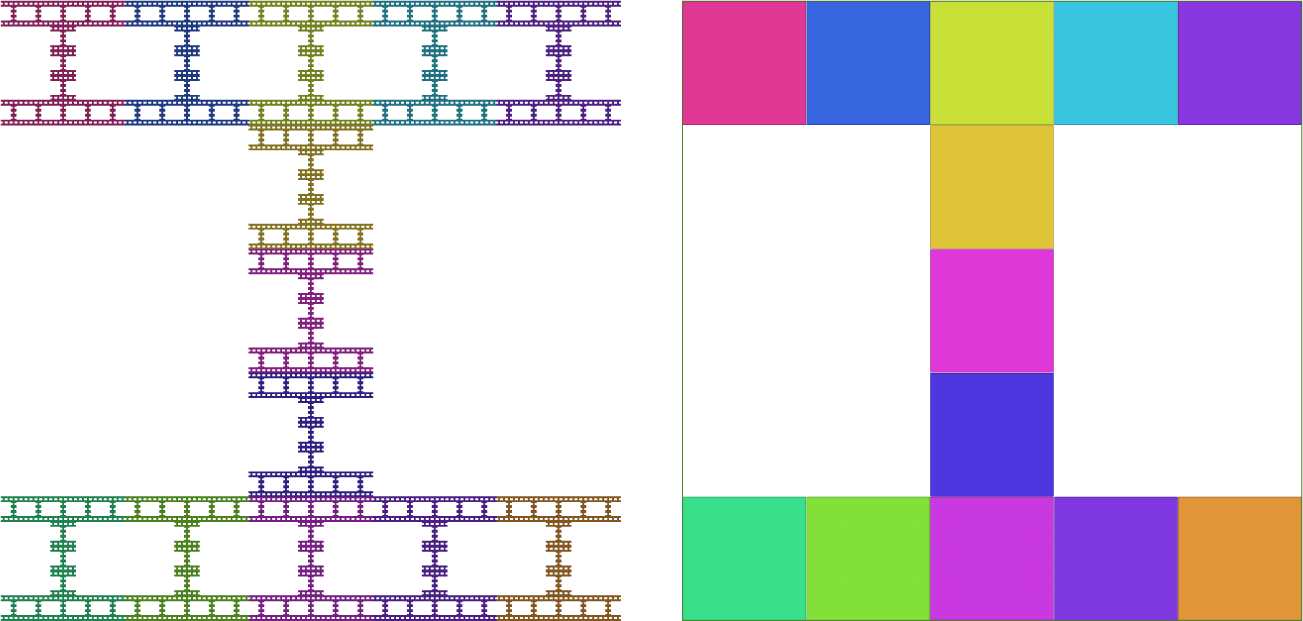
\includegraphics[width=0.8\textwidth]{line_int.png}
 \caption{Фрактальный квадрат с пересечением по полной стороне.}
 \label{fig:line_int}
\end{figure}

Поскольку любой фрактальный квадрат, являющийся дендритом, является множеством с одноточечным пересечением, то его двудольный граф пересечений может быть только деревом:

\begin{corollary}\label{cor:fsden}
Фрактальный квадрат $K$ является дендритом тогда и только тогда, когда его двудольный граф пересечений является деревом.\hfill\qed
\end{corollary}


\subsection{Самоподобная граница фрактального квадрата}

Рассмотрим множество $A=\{-1,0,1\}^2$ и соответствующее ему множество граней квадрата. 
Для фрактального квадрата $K$ с множеством единиц $D$ мы определим множество 
$$A_D=\{\bma\in A\mmm\{(0,0)\}: D\cap(D+\bma)\neq\0,\ F_\bma\neq\0\}.$$ 
Очевидно, что если $\bma\in A_D$, то и $-\bma\in A_D$.

Итак, множество $A_D$ --- это множество тех $\bma\in A$, для которых существуют копии $K_i, K_j$ такие, что $d_j-d_i=\bma$ и имеющие общие граничные точки. 
Для таких копий их общая граница равна $S_i(F_\bma)=S_j(F_{-\bma})$.\\

Следующее утверждение очевидно:

\begin{proposition}\label{prop:dd}
Самоподобная граница $\dd K$ фрактального квадрата $K$ есть объединение
$$\dd K=\bigcup\limits_{\bma\in A_D}F_\bma.$$
Если при этом $K$ --- дендрит, то для любого $\bma\in A_D$ множество $F_\bma$ одноточечно.
\end{proposition}

Заметим, что для любой копии $K_\bi$ из $K$ топологическая граница $K_\bi$ в $K$ является подмножеством в 
$S_\bi(\dd K)$. 
Таким образом, если путь $\ga\IN K$ имеет концы $a\in K_\bi$ и $b\in K\mmm K_\bi$, то $\ga$ содержит точку из $S_\bi(\dd K)$.

\begin{theorem}\label{ssboundary}
%Пусть $K$ --- фрактальный квадрат, являющийся дендритом и не являющийся отрезком. 
%Существуют следующие типы самоподобных границ $\dd K$:\\
%Если $\dd K=F_\bma\cup F_{-\bma}\cup F_\bmb\cup F_{-\bmb}$ то $\dd K$ будем относить к:\\
%типу {\bf A}, если $\bma=(1,0)$, $ \bmb=(0,1)$;\\ 
%типу {\bf B}, если $\bma=(1,1)$, $ \bmb=(1,-1)$; \\
%типу {\bf C}, если $\bma=\{(1,1),\ (1,-1)\},\bmb=\{(1,0),\ (0,1)\}$; или\\
%типу {\bf D}, если $\dd K=F_{(1,0)}\cup F_{(-1,0)}\cup F_{(0,1)}\cup F_{(0,-1)}\cup F_\bmb\cup F_{-\bmb}$,\\ 
%где $\bmb=(\be_1,\be_2)=\{(1,1),\ (1,-1)\}$.
% 
%Для типов {\bf A, B, C} множество $\#\dd K=4$. 
%Для типа {\bf D} либо $\#\dd K=6$ (обозначим такой случай как тип {\bf D6}), либо $\#\dd K=3$ (обозначим такой случай как тип {\bf D3}).
Пусть $K$ --- фрактальный квадрат, являющийся дендритом и не являющийся отрезком.
Тогда $\#\dd K\in\{3,\ 4,\ 6\}$. \\
%Самоподобная граница $\dd K$ может иметь только вид {\bf A, B, C} или {\bf D}:
 Если $\#\dd K=4$, то  $\dd K=F_\bma\cup F_{-\bma}\cup F_\bmb\cup F_{-\bmb}$, где   пара  $\bma,\bmb$ принимает одно из следующих значений:
	\begin{itemize}
	\item[{\bf A.}] $\bma=(1,0)$, $ \bmb=(0,1)$;
	\item[{\bf B.}] $\bma=(1,1)$, $ \bmb=(1,-1)$;
	\item[{\bf C.}] $\bma\in\{(1,1),\ (1,-1)\},\bmb\in\{(1,0),\ (0,1)\}$.
	\end{itemize}
 Если $\#\dd K=3$ или $\#\dd K=6$, то %самоподобная граница $\dd K$ имеет вид
\begin{itemize}
	\item[{\bf D.}] $\dd K=F_{(1,0)}\cup F_{(-1,0)}\cup F_{(0,1)}\cup F_{(0,-1)}\cup F_\bmb\cup F_{-\bmb}$, где $\bmb\in\{(1,1),\ (1,-1)\}$.
	\end{itemize}
\end{theorem}

В зависимости от выбора перечисленных  вариантов, мы будем говорить что $\dd K$ принадлежит к типу {\bf A,B,C} или {\bf D}.

\begin{remark}
Случай {\bf D} с $\#\dd K=6$ обозначим как {\bf D6}, а случай с $\#\dd K=3$ обозначим как {\bf D3}.
Случай {\bf D3} возникает, если существуют $\bma\in\{(1,0),(-1,0)\}$ и $\bmb\in\{(0,1),(0,-1)\}$ такие, что $F_\bma=F_\bmb$.
\end{remark}

\begin{figure}[H]
\centering
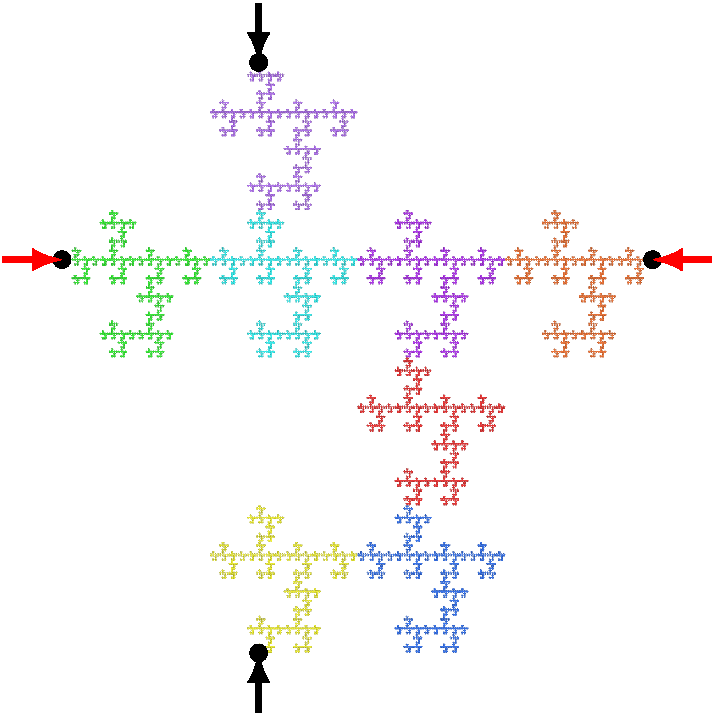
\includegraphics[width=0.3\textwidth]{A_type.pdf}
\hfill
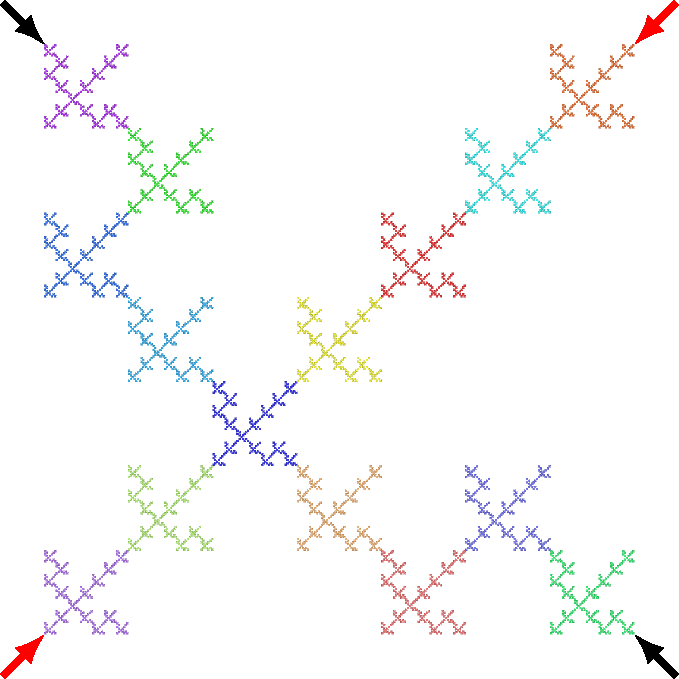
\includegraphics[width=0.3\textwidth]{B_type.pdf}
\hfill
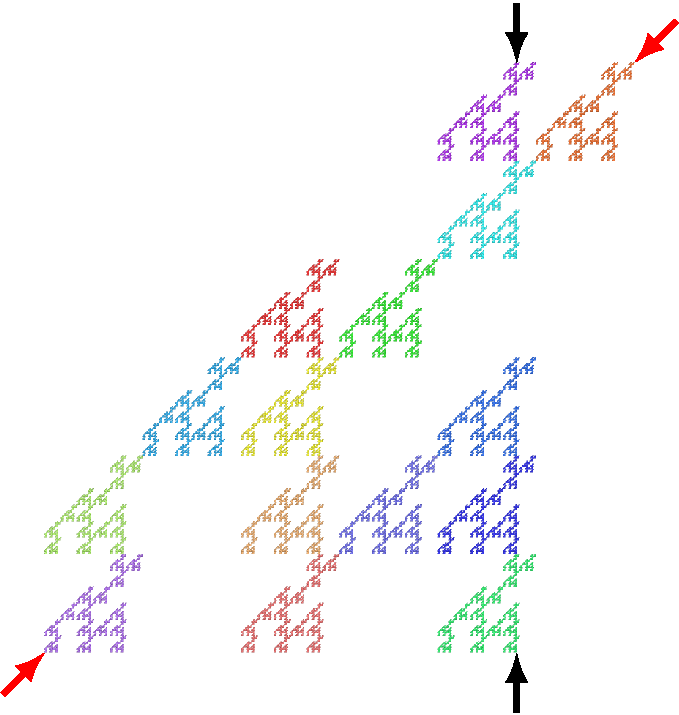
\includegraphics[width=0.3\textwidth]{C_type.pdf}
\caption{Фрактальные квадраты типа {\bf A}, {\bf B}, {\bf C}. Стрелки одного цвета указывают пару противоположных точек самоподобной границы, соответствующих одноточечным множествам $F_\bma$ и $F_{-\bma}$. }
\end{figure}

\begin{figure}[H]
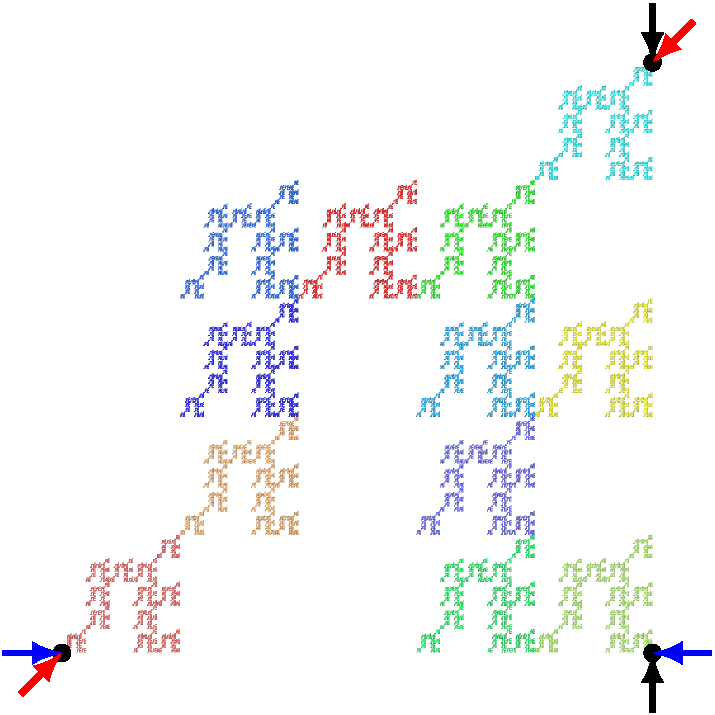
\includegraphics[width=0.3\textwidth]{D3_type.pdf}
\hfill
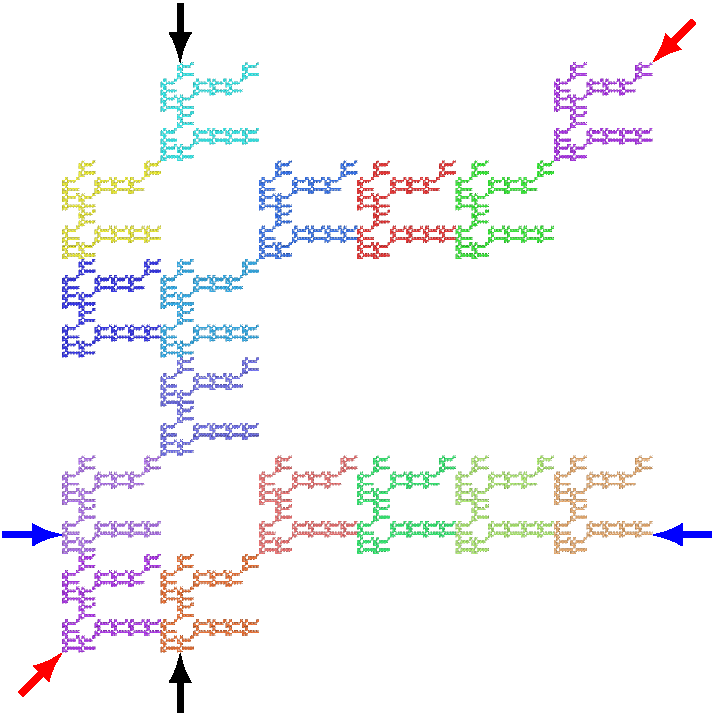
\includegraphics[width=0.3\textwidth]{D6_type.pdf}
\hfill
\caption{Фрактальные квадраты типа  {\bf D3} и {\bf D6}.  В типе {\bf D3} каждая точка самоподобной границы соответствует двум совпадающим множествам из системы $\{F_\bma\ :\ \bma\in A_D\}$.}
\end{figure}

\begin{proof}
Рассмотрим случай, когда самоподобная граница состоит из двух точек, то есть $\dd K=F_\bma\cup F_{-\bma}$ для некоторого $\bma\in A\mmm\{0\}$.
В этом случае $K$  есть отрезок с концами из $F_\bma$ и $ F_{-\bma}$.
Значит, у фрактального квадрата $K$, являющегося нетривиальным дендритом, $\#\dd K>2$.\\

Теперь покажем, что у фрактального квадрата $K$, являющегося (нетривиальным) дендритом, не может быть самоподобной границы, не относящейся к типам {\bf A, B, C, D}.
Нам достаточно показать, что если самоподобная граница имеет вид $\dd K=F_{(1,1)}\cup F_{(-1,-1)}\cup F_{(-1,1)}\cup F_{(1,-1)}\cup F_{(1,0)}\cup F_{(-1,0)}\cup F_{(0,1)}\cup F_{(0,-1)}$ или $\dd K=F_{(1,1)}\cup F_{(-1,-1)}\cup F_{(-1,1)}\cup F_{(1,-1)}\cup F_\bma\cup F_{-\bma}$, где $\bma\in\{(1,0),\ (0,1)\}$, то фрактальный квадрат не является дендритом.
Все эти случаи подразумевают, что $\{(0,0),\ (n-1,0),\ (0,n-1),\ (n-1,n-1)\}\IN D$, а значит, для каждого $\bma\in\{(1,0),\ (-1,0),\ (0,1),\ (0,-1)\}$ множество $F_\bma$ имеет мощность континуума (согласно Теореме \ref{fin_int}).
Это невозможно, поскольку такие $F_\bma$, согласно Предложению \ref{thm:den_necessary_sufficient}, должны быть одноточечными.\\

{\bf (A)} Для типа {\bf A} множество $\dd K$ может состоять только из четырёх точек. 
Если хоть одна из этих точек является угловой (углом квадрата), то $\dd K$ содержит ровно две угловых точки, которые являются концами некоторой стороны квадрата $P$, и три точки из $\dd K$ лежат на этой грани (см. первые два примера на рис. \ref{fig:tree3}).

Предположим, что $\dd K$ состоит из трёх точек.
Это возможно, только если эти точки являются угловыми (т.е. углами единичного квадрата), например, $(1,0),\ (0,0)$ и $(0,1)$.
Отсюда следует, что $F_{(1,-1)}\neq\0$.
%Если это так, то множество $\dfrac{D+P}{n}$ связно и содержит точки $(1,0)$ и $(0,1)$. 
Мы утверждаем, что в этом случае $G_{(1,-1)}=(D\cap (D+(1,-1))\neq\0$.
Действительно, пусть $D'$ --- подмножество в $D$, удовлетворяющее условиям:\\
1. Множество $D'+P$ связно;\\
2. $D'\cap (D'+(1,-1))=\varnothing$;\\
3. $(0,n-1)\in D'$. \\
Тогда $D'$ равно либо $\{0\}\times\{k,\ldots,n-1\}$, либо $\{k,\ldots,n-1\}\times\{n-1\}$ для некоторого $0\leq k\leq n-1$.
Поскольку $D'+P\IN D+P$ и $D+P$ связно, существует $d\in D$ такое, что $d\in D'+(1,-1)$, поэтому $G_{(1,-1)}\neq\0$.
%Это наблюдение доказывает наше утверждение.
Итак, из $F_{(1,-1)}\neq\0$ и $(1,-1)\in A_D$ следует, что $\dd K$ относится к типу {\bf D}. \\

{\bf (B)} Для типа {\bf B} очевидно, что $\#\dd K=4$, поскольку $\dd K=\{(0,0),\ (1,0),\ (0,1),\ (1,1)\}$.\\

{\bf (C)} Рассуждая аналогично случаю {\bf (A)}, легко увидеть, что для типа {\bf C} множество $\dd K$ также состоит ровно из четырёх точек. \\

{\bf (D)} Пусть для типа {\bf D} граница $\dd K=F_{(1,0)}\cup F_{(-1,0)}\cup F_{(0,1)}\cup F_{(0,-1)}\cup F_{(1,1)}\cup F_{(-1,-1)}$.
Пусть $\bma\in\{(1,0),(-1,0)\}$ и $\bmb\in\{(0,1),(0,-1)\}$.
Тогда равенства $F_\bma=F_{-\bmb}$, $F_{\bmb}=F_{\bma+\bmb}$ и $F_{-\bma}=F_{-\bma-\bmb}$ эквивалентны и $\dd K=F_{-\bma}\cup F_\bma\cup F_\bmb$. 

Значит, если объединение $\dd K=F_{(1,0)}\cup F_{(-1,0)}\cup F_{(0,1)}\cup F_{(0,-1)}\cup F_{(1,1)}\cup F_{(-1,-1)}$ является дизъюнктным, то $\#\dd K=6$, в противном случае $\#\dd K=3$.
%Это показывает что для типа {\bf D} из $\#\dd K<6$ следует . 
%Обозначим получившиеся два подтипа как {\bf D3} и {\bf D6}.
\end{proof}


\section{Порядок точек ветвления фрактального квадрата, являющегося дендритом}

\subsection{Запретные комбинации в множествах единиц для разных типов фрактальных квадратов, являющихся дендритами}

Для фрактального квадрата, являющегося дендритом, можно указать комбинации единиц, которые не могут встречаться в $D^k$ для любого $k$. 
В следующей лемме рассматриваются такие комбинации. 
Мы говорим, что множество $Q\IN \zz^2$ {\em  запретное} (для фрактального квадрата $K$ с самоподобной границей данного типа), если для любых $k\in\nn$ и $\widetilde d\in D^k$ верно
$\widetilde d+Q\not\IN D^k.$

\begin{lemma}\label{quadruples}
Следующие комбинации единиц $Q$ запретные:
\begin{itemize}[nolistsep]
\item[(1)] $\{(0,0), (1,0)\} $ и $\{(0,0), (0,1)\} $ для типа {\bf B};
\item[(2)] $\{(0,0), (0,1), (1,0), (1,1)\}$ для типов {\bf A, B, D};
\item[(3)] $\{(0,0),\bma,\bmb,\bma+\bmb\}$ для типа {\bf C};
\item[(4)] тройка $\{a_1, a_2, a_3\}$ для типа {\bf D3}, если $\dd K=\{a_1,a_2, a_3\}$;
\item[(5)] тройки $\{(0,0),(\be_1,0),\bmb\}$ и $\{(0,0),(0,\be_2),\bmb\}$ для типа {\bf D6}. 
\end{itemize}
\end{lemma}

\begin{proof} 
%Чтобы доказать, что множество $Q$ целочисленных векторов является {\em запретным} в каждом из случаев, мы убедимся, что множество $Q+K$ содержит замкнутые контуры.

Случай (1) очевиден, так как для любого $\bma\in\{(0,1),(1,0)\}$ множество $F_\bma$ несчётно.
Эта запретная комбинация также встречается в случае (2) для типа {\bf B}.\\

Чтобы доказать, что множество $Q$ целочисленных векторов {\em запретное} для типов {\bf A, C, D}, мы убедимся, что множество $Q+K$ содержит нестягиваемую замкнутую  кривую.\\

(2)  Рассмотрим тип {\bf A} и множество $Q=\{(0,0), (0,1), (1,0), (1,1)\}$. 
Мы положим, что $\bma=(1,0), \bmb=(0,1)$. 
Тогда   либо $F_{-\bma}=\{(0,b)\}, F_{-\bmb}=\{(a,0)\}$, где $a,b$ принадлежат интервалу $]0,1[$,  либо в случае {\bf A} только одно из значений $a,b$, скажем $b$, равно $0$.

В первом случае, поскольку одно из множеств $F_{(1,1)}$ или $F_{(1,-1)}$ пусто, существует открытый квадрат $\dot P_x:=\dfrac{x+\dot P}{n}$, $x\in \{(-1,-1),(0,-1), (-1,0), (0,0)\}$ который имеет пустое пересечение с $Q+K$. 

Обозначим $x_1=(a,0)$, $x_2=(0,b)$, $x_3=(a-1,0)$, $x_4=(0,b-1)$. 

В множествах  $K$, $-\bma+K$, $-\bma-\bmb+K$ и $-\bmb+K$ содержатся поддуги  $\ga(x_1,x_2)$, $\ga(x_2,x_3)$,$\ga(x_3,x_4)$ и $\ga(x_4,x_1)$ соответственно. 
Их объединение образует замкнутую кривую, лежащую в $Q+K$ и обходящую $\dot P_x$, поэтому эта дуга не стягиваема (см. рисунок \ref{forbid} {\bf A}).\\ 

Если же для типа {\bf A} имеем $F_{-\bma}=(0,0)$, а квадрат $\dot P_x$ имеет пустое пересечение с $Q+K$ для каждого $x\in\{(-1,0), (0,0)\}$, то рассуждения остаются аналогичными (см. рисунок \ref{forbid} {\bf A*}).\\

\begin{figure}[h] 
    \centering
    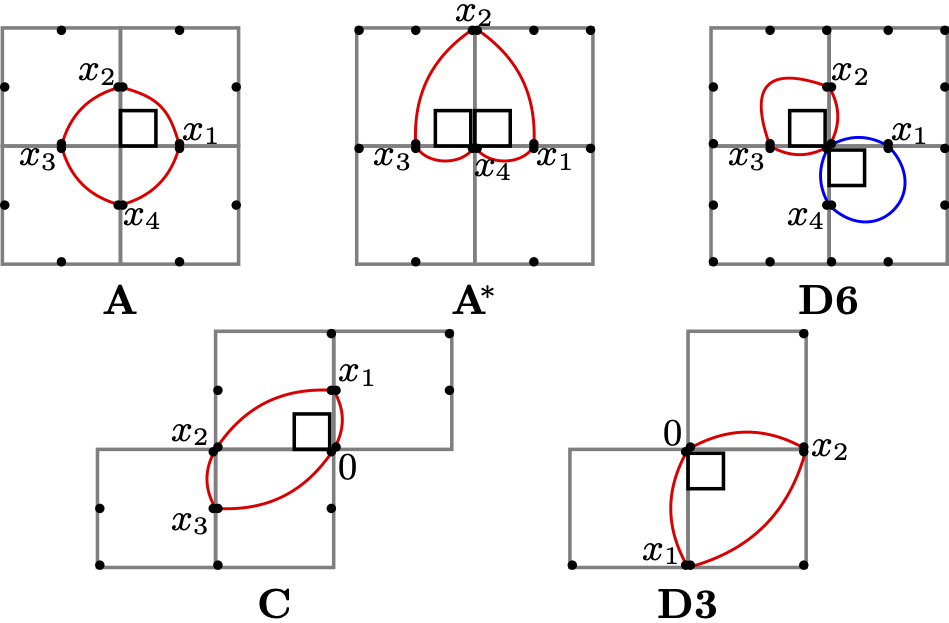
\includegraphics[width=.8\textwidth]{quadruples.png}
    \caption{Построение нестягиваемых петель в запретных комбинациях для типов {\bf A, C} и {\bf D}.}
    \label{forbid}
\end{figure}

Аналогичным образом доказываются утверждения (3), (4) и (5).
Мы выбираем вершину в $Q+K$, около которой существует открытый квадрат $\dot P_x$, имеющий пустое пересечение с $Q+K$, и теперь формируем нестягиваемую петлю из поддуг $\ga(x_i,x_j)$, соединяющих граничные точки множеств $q_i+K$.
Выбор точек и дуг показан на рисунке \ref{forbid}.
\end{proof}


\subsection{Порядок ветвления точки фрактального квадрата}

\begin{lemma}\label{thm:vertex_branching}
Пусть $K$ --- фрактальный квадрат, являющийся дендритом.
Для любой угловой точки $a\in K$,
 $Ord(a,K)\leq 2$.
\end{lemma}

\begin{figure}[h!]
\centering
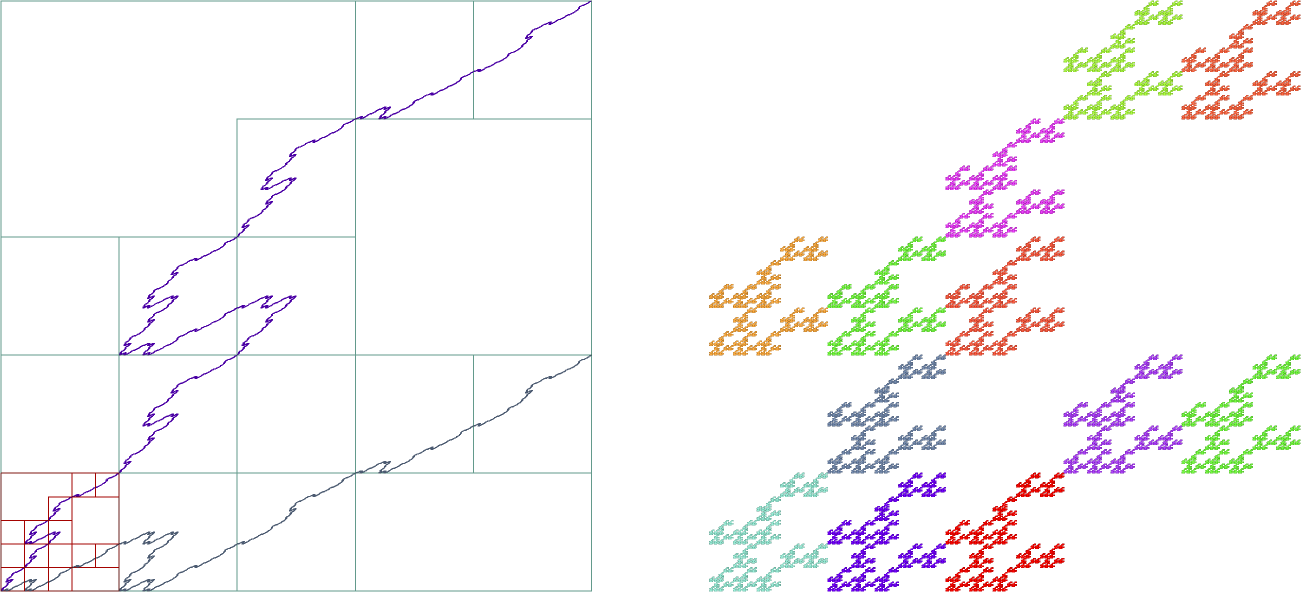
\includegraphics[width=0.7\textwidth]{C_type_Three.png}
\caption{Угловая точка порядка 2 для типа {\bf C} и две главные дуги, содержащие ее.} 
\label{fig:C_type_Three}
\end{figure}

\begin{proof}\label{proof:vertex_branching}
Заметим, что если копия $K_\bi$ содержит угловую точку $a$, то 
$K_\bi\mmm \{a\}=S_\bi(K\mmm \{a\})$, поскольку $a$ --- неподвижная точка гомотетии $S_\bi$.
Следовательно, если $Q$ является компонентой в $K\mmm \{a\}$, то $Q\cap K_\bi=S_\bi(Q)$. 
Пусть $\{Q_1,\ldots, Q_k\}$ --- множество всех этих компонент, тогда $K\mmm \{a\}=\bigsqcup \limits_{j=1}^kQ_j$ и $\dd K\mmm \{a\}=\bigsqcup \limits_{j=1}^k(Q_j\cap\dd K)$, поэтому $\dd K_\bi\mmm \{a\}=\bigsqcup \limits_{j=1}^k(Q_j\cap\dd K_\bi)$. 
Число $k$ пересечений в последнем равенстве не больше чем $3$, так как эти пересечения соответствуют двум сторонам и одной вершине, противоположным точке $a$. 
Каждое из этих пересечений содержит не более одной точки, и то же самое верно для соответствующих пересечений $Q_j\cap\dd K$.

Без потери общности предположим, что  $a=(0,0)$.
Таким образом,\\ 
$Q_1\cap\dfrac{K+(1,0)}{n} =\dfrac{F_{(1,0)}}{n}$,\quad если $(1,0)\in D$;\\
$Q_2\cap\dfrac{K+(0,1)}{n} =\dfrac{F_{(0,1)}}{n}$,\quad если $(0,1)\in D$;\\ 
$Q_3\cap\dfrac{K+(1,1)}{n} =\dfrac{F_{(1,1)}}{n}$,\quad если $(1,1)\in D$.
% $Q_2\cap K_{01}=F_{01}$ если $d_{(0,1)}\in D$ и $Q_3\cap K_{11}=F_{11}$ если $d_{(1,1)}\in D$.

\noindent 
Для типа {\bf A} имеем $F_{(1,1)}=\0$, поэтому $Ord(a,K)\leq 2$.\\
Для типа {\bf B} верно $D\not\ni\{(1,0),(0,1)\}$, следовательно $Ord(a,K)=1$.\\
Для типа {\bf C} либо $F_{(1,0)}=\0$, либо $F_{(0,1)}=\0$, следовательно $Ord(a,K)\leq 2$.

Предположим, что для типа {\bf D} порядок угловой точки $a=(0,0)$ равен $3$.
Тогда $\{(0,0),\ (1,0),\ (0,1),\ (1,1)\}\in D$. 
По Лемме \ref{quadruples}, это невозможно.
Это противоречие показывает, что для типа {\bf D}, $Ord(a,K)\leq 2$.
\end{proof}

Далее определим, сколько угловых точек может быть у фрактального квадрата с самоподобной границей границей каждого из типов: {\bf A, B, C, D3, D6}.

\begin{theorem}\label{thm:corner}
Пусть $K$ --- фрактальный квадрат, являющийся дендритом.
\begin{itemize}[nolistsep]
\item[(A)] Если $K$ имеет границу типа  {\bf A}, то у него может быть
	\begin{itemize}[nolistsep]
	\item[(a.1)] две угловые точки с порядками ветвления $2,1$ или $1,1$;
	\item[(a.2)] одна угловая точка с порядком ветвления $\le 2$; или 
	\item[(a.3)] могут вовсе отсутствовать угловые точки.
	\end{itemize}
\item[(B)] Если $K$ имеет границу типа  {\bf B}, то $K$ имеет четыре угловые точки с порядком ветвления $1$.
\item[(C)] Если $K$ имеет границу типа {\bf C}, то $K$ имеет две угловые точки, порядки ветвления которых $\le 2$.
\item[(D)] Если же $K$ имеет границу типа {\bf D}, то он может иметь 
	\begin{itemize}[nolistsep]
	\item[(d.1)] две угловые точки порядков $\le 2$ для подтипа {\bf D6}; или
	\item[(d.2)] три угловые точки порядка $1$ для подтипа {\bf D3}
	\end{itemize}
\end{itemize}
\end{theorem}

\begin{proof}

Отметим, что наличие угловых точек $(0,0), (1,0), (0,1)$ или $(1,1)$ в $K$ равносильно наличию в $D$  векторов $(0,0), (n-1,0), (0,n-1)$ или $(n-1,n-1)$ соответственно.
\\

(A) Согласно теореме \ref{ssboundary}, если $K$ имеет самоподобную границу типа {\bf A}, то $K$ не может содержать пару противоположных угловых точек. 
Поэтому $K$ содержит не более двух угловых точек, которые являются концами некоторой стороны квадрата $P$. 
Пусть этими двумя точками являются $(0,0)$ и $(1,0)$, тогда $\dd K=\{(0,0),\ (a,0),\ (1,0),\ (a,1)\}$, где $a\in]0,1[$. 

Если порядки обеих точек, $(0,0)$ и $(1,0)$,  равны $2$, то $\{(0,1),\ (1,0),\ (n-2,0),\ (n-1,1)\}\IN D$, поскольку каждая из копий $\frac{K}{n}$ и $\frac{(0,n-1)+K}{n}$ должна иметь двух соседей (см. рисунок \ref{fig:corner} слева). 
В этом случае $\#G_{(1,0)}\geq2$, следовательно $F_{(1,0)}$ несчётно, что невозможно, поскольку $F_{(1,0)}\IN\dd K$ и $G_{0(1,0)}$.
Следовательно, порядки ветвления этих двух точек могут быть равны $2,1$ или $1,1$.\\

(B) Из Теоремы \ref{ssboundary} следует, что $K$ содержит $4$ угловые точки тогда и только тогда, когда $\dd K$ относится к типу {\bf B}.
Согласно лемме \ref{thm:vertex_branching}, порядки ветвления этих точек равны 1.\\

(C, d.1) Если $K$ имеет ровно $2$ угловые точки, являющиеся противоположными, то $\dd K$ относится к типу {\bf C} или {\bf D6}.
Их порядки ветвления, согласно лемме \ref{thm:vertex_branching}, не превышают $2$.
\begin{figure}[H]
\centering
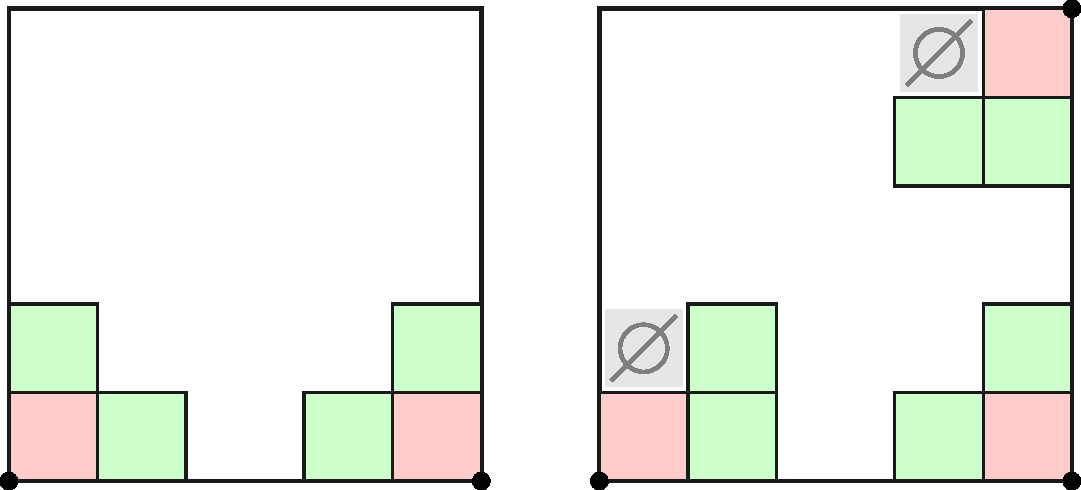
\includegraphics[width=0.8\textwidth]{corner.pdf}
\caption{На рисунках слева и по центру показаны для фрактальных квадратов с самоподобной границей типа {\bf A} или {\bf D3} их угловые точки, содержащие их угловые копии (красные) и возможные соседствующие копии для угловых копий (зелёные).
}
\label{fig:corner}
\end{figure}

(d.2) Согласно теореме \ref{ssboundary}, $K$ имеет $3$ угловые точки тогда и только тогда, когда $\dd K$ относится к типу {\bf D3}.
Предположим, не ограничивая общности, что угловыми точками в $K$ являются $(0,0)$, $(1,0)$ и $(1,1)$.

Если $(0,1)\in D$, то при $\bma=(-1,0)$ и $\bmb=(-1,-1)$ мы получим $(0,0)\in G_\bma$ и $(0,1)\in G_{\bma\bmb}$.
Но тогда, согласно теореме \ref{fin_int}, $F_\bma$ содержит $\{(0,0)\}\cup\bigcup\limits_{m=0}^\8 S^m(F_\bmb)$, где $S(x)=\frac{x+(1,0)}{n}$ и $F_\bmb=\{(0,0)\}$.
Поэтому множество $F_\bma$ бесконечно и не совпадает с $\{(0,0)\}$.

Чтобы показать, что $G_{0\bma}\neq\0$, допустим противное.
Если в графе пересечений $\tilde\Ga$ для $K$ в качестве вершин взять точки из $D$ на плоскости, то его рёбрами могут быть только отрезки, конгруэнтные векторам $(0,1)$ и $(1,1)$.
При этом в $D$ не должно быть пары точек, разность координат которых равна $(1,0)$.
Тогда любая ломаная, которая содержит точку $(0,0)$, лежит в полуплоскости $y\ge x$ и поэтому не содержит точку $(n-1,0)$.
Следовательно, граф $\tilde\Ga$ несвязен, что невозможно.
%Тогда копию $\frac{K}{n}$ с копией $\frac{K+(n-1,n-1)}{n}$ соединяет только только цепочка копий $\left\{\frac{K+(p,p)}{n}\right\}_{p=1}^{n-2}$.
%Аналогично, копию $\frac{K+(n-1,0)}{n}$ можно соединить с копией $\frac{K+(n-1,n-1)}{n}$ только цепочкой копий $\left\{\frac{K+(n-1,p)}{n}\right\}_{p=1}^{n-2}$.
%Но тогда $\frac{K+(n-2,n-2)}{n}\cap\frac{K+(n-1,n-2)}{n}=\frac{F_\bma+(n-1,n-2)}{n}$, то есть $(n-1,n-2)\in G_{0\bma}$ (на рисунке \ref{fig:corner} справа эти копии обведены синим контуром).

Аналогично получаем бесконечное $F_{(0,1)}$ при $(n-2,n-1)\in D$.
Поэтому $(0,1)\notin D$ и $(n-2,n-1)\notin D$. 
 
Если $Ord((0,0),K)=2$, то у копии с единицей $(0,0)$ есть $2$ соседа. 
Следовательно, $\{(0,0),\ (1,0),\ (1,1)\}\IN D$, но эта комбинация единиц является запретной.
Аналогично, точки $(1,0), (1,1)$ не могут иметь порядок $2$, поскольку соответствующие комбинации $\{(n-1,0),\ (n-2,0),\ (n-1,1)\}$ и $\{(n-1,n-1),\ (n-2,n-2),\ (n-1,n-2)\}$ являются запретными. 
\end{proof} 

% The Figures \ref{fig:A_type_Three}, \ref{fig:C_type_Three} and
% \ref{fig:D6_type_Three} show the corner points of  order two for the types {\bf A, C, D6} respectively.
% \begin{figure}[H]
%     \centering
%     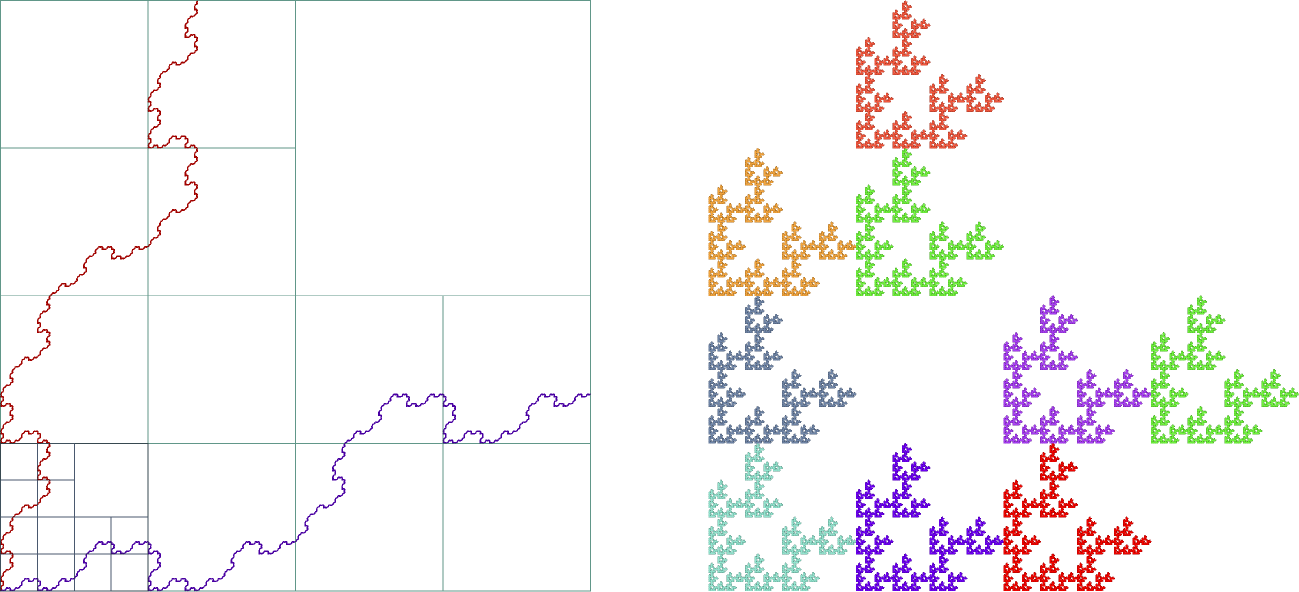
\includegraphics[width=0.7\textwidth]{A_type_Three.png}
%     \caption{}
%     \label{fig:A_type_Three}
% \end{figure}

% \begin{figure}[H]
%     \centering
%     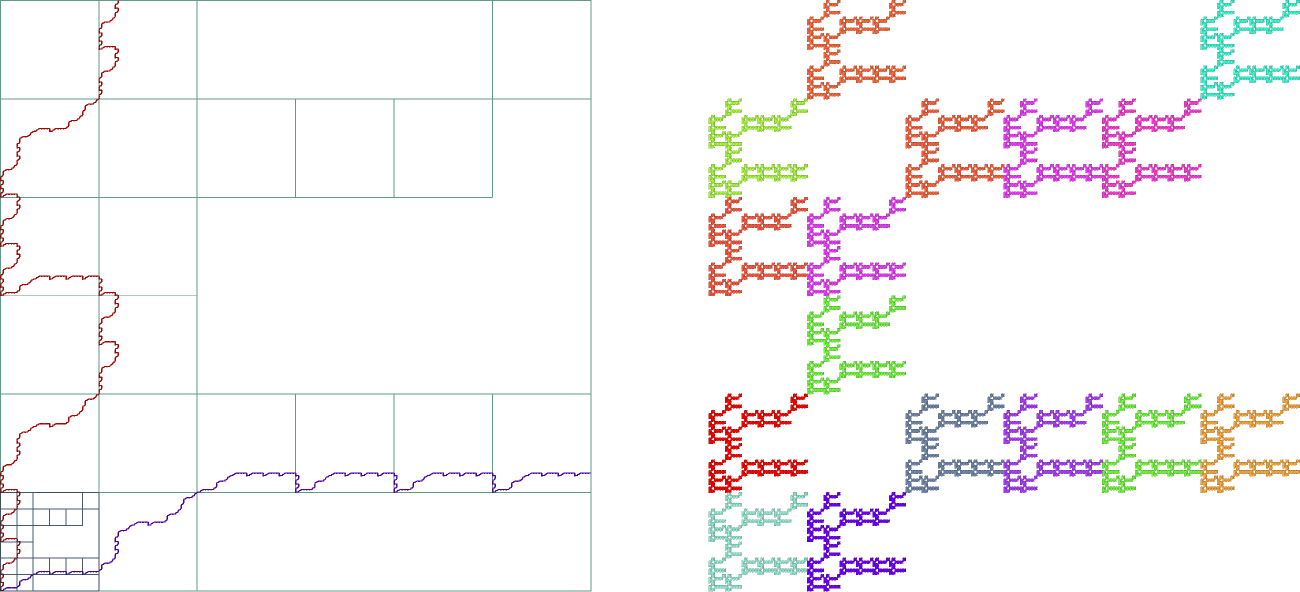
\includegraphics[width=0.7\textwidth]{D6_type_Three.png}
%     \caption{}
%     \label{fig:D6_type_Three}
% \end{figure}

\begin{theorem}\label{order}
Пусть $K$ --- фрактальный квадрат, являющийся дендритом. 
Тогда $Ord(x,K)\le 4$ для любого $x\in K$.\\
Если $\dd K$ типа {\bf D} и $x\notin S_\bi(\dd K)$ для любого $\bi\in I^*$, то $Ord(x,K)\le 3$.\\
Если $\dd K$ типа {\bf D3} и $x\in \dd K_\bi$ для некоторого $\bi\in I^*$, то $Ord(x, K)\le 3$.
\end{theorem}

\begin{proof}\label{proof:point_branching}
Пусть $Ord(x,K)=l$.
Тогда существуют такие $l$ жордановых дуг $\{\ga_i\}_{i=1}^l$ в $K$ с общим концом $x$, что дуги $\ga_i\mmm \{x\}$ не пересекаются.
Существует такое $p\in\nn$, что для каждой дуги $\ga_i$ справедливо неравенство $|\ga_i|>\sqrt{2}n^{-p}$.
Из леммы \ref{quadruples} следует, что существуют $1$, $2$ или $3$ мультииндекса $\bi=i_1i_2\ldots i_p$ таких, что $x\in S_\bi(K)$.\\

\textbf{(1)} В случае, когда такой $\bi$ единственен, то есть $x\in \dot K_\bi$, каждая дуга $\{\ga_i\}$ проходит в одну из соседних для $K_\bi$ копий порядка $p$ через одну из точек $\dd K_\bi$ (см. рисунок \ref{fig:case1}). 
Таким образом, число $l$ не превышает количества соседей для $K_\bi$  и числа точек в $\dd K_\bi$. 
По теореме \ref{ssboundary}, для типов {\bf A, B, C} число $l\leq 4$.

Для типа {\bf D} получаем $l\le 3$, так как при выборе любых четырёх из шести возможных соседей копии $K_\bi$, мы получаем запретную комбинацию.

\begin{figure}[H]
\centering
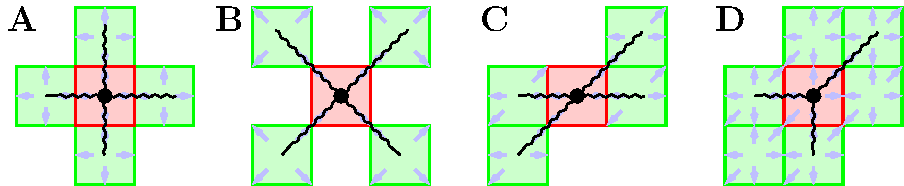
\includegraphics{case1.pdf}
\caption{Копия с $x\in\dot K_\bi$ (красная) и возможные соседи (зелёные) в типах \textbf{A}, \textbf{B}, \textbf{C} и \textbf{D}}
\label{fig:case1}
\end{figure}

\textbf{(2)} Рассмотрим случай, когда $x\in K_\bi\cap K_\bj$ и $x$ лежит внутри (не на конце) общего ребра квадратов $S_\bi(P)$ и $S_\bj(P)$ .
Он возможен только для типов \textbf{A}, \textbf{C} и \textbf{D6} (см. рисунок \ref{fig:case2}).
В отличие от случая \textbf{(1)}, здесь $x\in S_\bi(\dd K)$.

В этой ситуации $l$ не превышает максимального числа соседей для пары копий, которые содержат $x$.
Согласно Лемме \ref{quadruples}, число соседей для $K_\bi\cup K_\bj$ не может превышать $4$.

\begin{figure}[H]
\centering
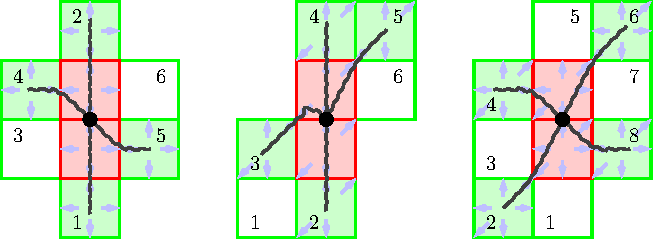
\includegraphics{case2.pdf}
\caption{Пара копий с $x$ на общей стороне (красные) и их возможные соседи (зелёные) для типов \textbf{A}, \textbf{C} и \textbf{D6}}. 
\label{fig:case2}
\end{figure}

\textbf{(3)} Рассмотрим случай, в котором $x$ является общей угловой точкой для двух или трех копий.
Пусть $x$ --- вершина для $S_\bi(P)$.
Для типов \textbf{A},  \textbf{B}, \textbf{C} и \textbf{D6} точка $x$ принадлежит не более чем двум копиям $K_\bi, K_\bj$, а в случае \textbf{D3} точка $x$ может принадлежать не более чем трём копиям $K_\bi, K_\bj, K_\bk$, как это показано на рисунке \ref{fig:case3}.

Согласно теореме \ref{thm:vertex_branching}, $Ord(x,K_\bi)\leq2$ для любой копии $K_\bi$.
Более того, для типов \textbf{B} и \textbf{D3} порядок угловой точки относительно копии равен $1$.
Тогда $Ord(x,K_\bi\cup K_\bj)\leq2$ для типа \textbf{B} и $Ord(x,K_\bi\cup K_\bj\cup K_\bk)\leq3$ для типа \textbf{D3}.
Следовательно, $Ord(x,K)\leq3$ для типа {\bf D3} и $Ord(x,K)\leq2$ для типа {\bf B}.

Число $l$ не превышает максимального числа соседей для копий, содержащих $x$.
Тогда для типов {\bf A, C, D6}, согласно лемме \ref{quadruples}, $Ord(x,K)\leq4$.
\end{proof}

\begin{figure}[H]
\centering
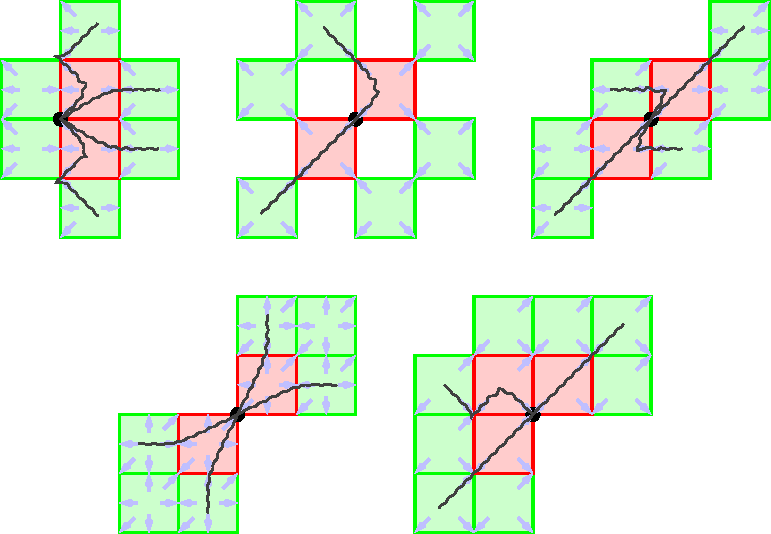
\includegraphics[width=0.6\textwidth]{case3.pdf}
\caption{Копии с общей угловой точкой $x$ (красные) и их возможные соседи (зелёные) для типов {\bf A, B, C, D6, D3}.}
\label{fig:case3}
\end{figure}


\section{Теорема о классификации фрактальных квадратов, являющихся дендритами}

Для доказательства основной теореме нам потребуется следующее утверждение о порядках ветвления точек относительно главного дерева.

\begin{proposition}\label{lem:d4bound}
Допустим, $K$ относится к типу {\bf D6} и $\gamma$ --- его главное дерево.
\begin{itemize}[nolistsep]
    \item[(i)] $Ord(x,\gamma)\leq2$ для любого $x\in\dd K$;
    \item[(ii)] $Ord(x,K)\leq3$ для любого $x\in\ga$.
\end{itemize}
\end{proposition}



\begin{proof}
(i). Для угловых точек в $K$ неравенство $Ord(x,\gamma)\leq2$ следует из Предложения \ref{thm:corner}.

Пусть $x\in\dd K$ не является угловой.
Из доказательства Теоремы \ref{order} следует, что порядок ветвления $x$ относительно $\ga$ меньше или равен числу соседей у копии $K_i$. 
Как показано на рисунке \ref{fig:case2}, у любой копии $K_i$, отмеченной на этом рисунке красным цветом, может быть не более двух соседей, в противном случае возникают запретные комбинации. 
Таким образом, $Ord(x,\gamma)\leq Ord(x,K)\leq2$.
\begin{figure}[H]
    \centering
    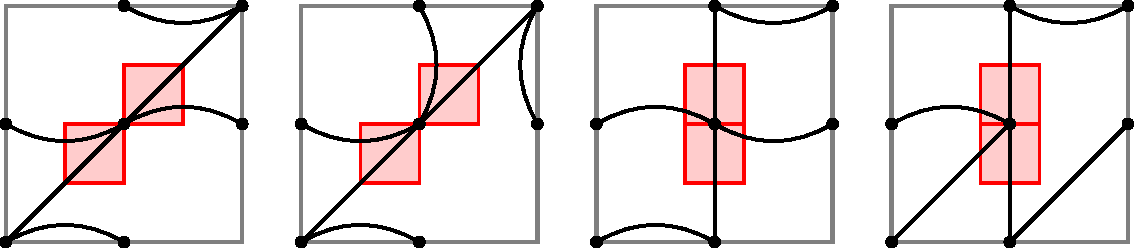
\includegraphics[width=\textwidth]{d6ord3full.pdf}
    \caption{Предполагаемые конфигурации главного дерева $\ga$ при допущении того, что $Ord(x,\gamma)=4$ для типа {\bf D6}. Точка $x$ располагается в центре.}
    \label{fig:d6ord3full}
\end{figure}

(ii)  Пусть существует $x\in\ga$ такое, что $Ord(x,\gamma)=4.$
Из Теоремы \ref{order} следует, что  $x=S_i(K)\cap S_j(K)$ для некоторых $i,j\in I$.\\
Рассмотрим сначала случай, когда $x$ является общей угловой точкой копий  $S_i(K)$ и $S_j(K)$, так что $x=S_i(b)=S_j(a)$, где $a=(0,0)$ и $b=(1,1)$. 
Так же обозначим $F_{0,-1}=\{c\}$, $F_{0,1}=\{d\}$, $F_{-1,0}=\{e\}$, $F_{1,0}=\{f\}$.

\begin{figure}[H]
    \centering 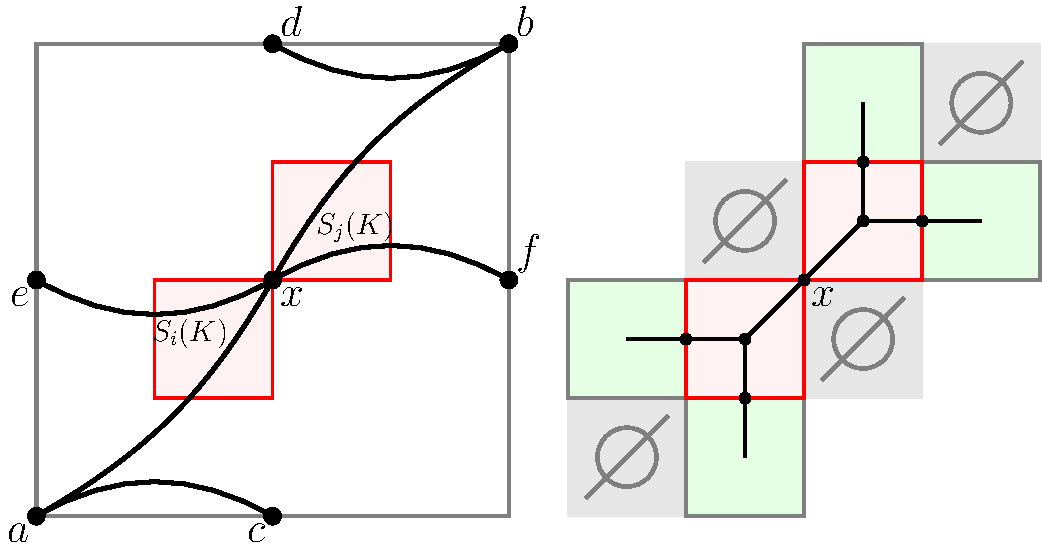
\includegraphics[width=0.7\textwidth]{d6ord3_12.pdf}
    % \caption{Caption}
    % \label{fig:d6ord3_12}
\end{figure}

Для точек $a,b$ согласно Теоремам \ref{thm:vertex_branching} и \ref{order} следует, что $Ord(a,\ga)=Ord(b,\ga)=2$. 
Тогда множество $\ga\mmm\{a,b\}$ состоит из трёх компонент. 
Обозначим замыкания этих компонент как $\ga_0$, $\ga_a$, $\ga_b$ так, чтобы $\ga_0\cap\ga_a=\{a\}$ и $\ga_0\cap \ga_b=\{b\}$. 
Компонента $\ga_0$ содержит дугу $\ga(a,b)$, которая делит $P$ на две части. 
В одной из них находятся точки $c$ и $f$, в другой --- $e$ и $d$, поэтому $x\in \ga(a,b)$ и множество $\ga_0$ содержит одну из пар точек: $\{c,d\}$, $\{c,f\}$, $\{e,f\}$ или $\{e,d\}$.

Рассмотрим случай, когда $\ga_0\NI\{e,f\}$. 
Тогда $\ga_a=\ga(a,c)$ и $\ga_b=\ga(b,d)$.

Следовательно множество $\ga_0$ является объединением поддуг $\ga(a,x)$, $\ga(f,x)$, $\ga(b,x)$ и $\ga(e,x)$.

Эти четыре поддуги пересекают множество $S_i(\dd K)\cup S_j(\dd K)$ в четырёх различных точках $S_i(c)$, $S_i(e)$, $S_j(f)$, $S_j(d)$. 
поэтому пересечение этих поддуг с $S_i( K)\cup S_j(K)$ должны быть различными поддугами $S_i(\ga(c,b))$,  $S_i(\ga(e,b))$, $S_j(\ga(f,a))$, $S_j(\ga(d))$, чьи внутренности лежат в разных компонентах множества $\ga_0\mmm\{x\}$. 
Это невозможно, так как $\ga(a,f)\cap\ga(a,d)=\ga(a,x)$.\\

Рассмотрим теперь случай, когда $x$ лежит на общей стороне двух копий $S_i(K)$ и $S_j(K)$. 
В этом случае $F_{0,-1}=\{c\}$, $F_{0,1}=\{d\}$, так что $x=S_i(d)=S_j(c)$.  
Обозначим $F_{-1,-1}=\{a\}$, $F_{1 ,1}=\{b\}$, $F_{-1,0}=\{e\}$, $F_{1,0}=\{f\}$.

Для точек $c,d$ из Теоремы \ref{thm:vertex_branching}, \ref{order} следует, что $Ord(c,\ga)=Ord(d,\ga)=2$. 

Поэтому множество $\ga\mmm\{c,d\}$  состоит из трёх компонент. 
Обозначим замыкания эти компонент как $\ga_0$, $\ga_c$, $\ga_d$ так, чтобы $\ga_0\cap\ga_c=\{c\}$ и $\ga_0\cap \ga_d=\{d\}$. 
Компонента $\ga_0$ содержит дугу $\ga(c,d)$, которая делит $P$ на две части. 
Одна из этих частей содержит точки $b$ и $f$, другая содержит $e$ и $a$, следовательно $x\in \ga(c,d)$, а множество $\ga_0$ содержит одну из пар точек: $\{a,b\}$, $\{a,e\}$, $\{e,f\}$ или $\{b,f\}$. 

\begin{figure}[H]
    \centering
    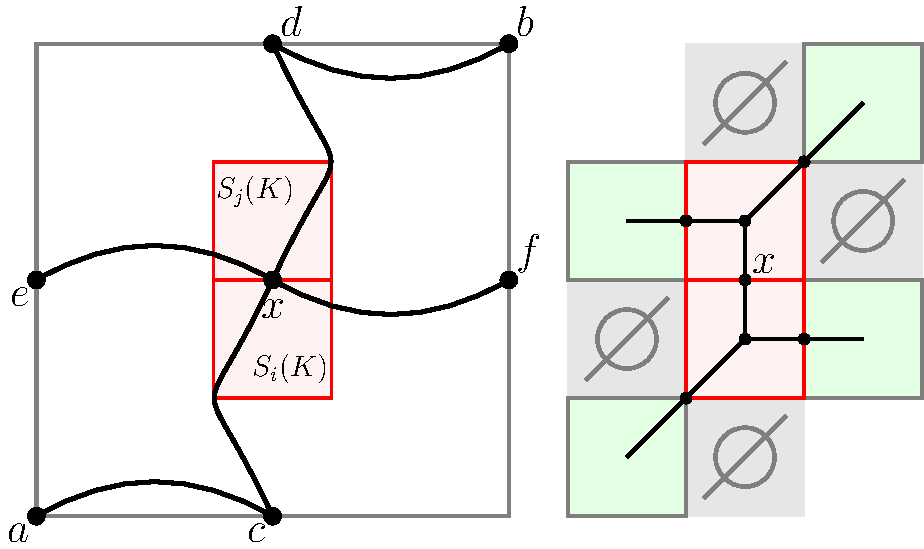
\includegraphics[width=0.65\textwidth]{d6ord3_34.pdf}
    % \caption{Caption}
    % \label{fig:d6ord3_34}
\end{figure}

Рассмотрим случай, когда $\ga_0\NI\{e,f\}$. 
Тогда $\ga_c=\ga(a,c)$ и $\ga_d=\ga(b,d)$.

Следовательно, множество $\ga_0$ является объединением поддуг  $\ga(c,x)$, $\ga(f,x)$, $\ga(d,x)$ и $\ga(e,x)$.

Эти четыре поддуги пересекают множество $S_i(\dd K)\cup S_j(\dd K)$ в четырёх различных точках: $S_i(e)$, $S_i(b)$, $S_j(f)$ и $S_j(a)$. 
Поэтому пересечения этих четырёх поддуг с $S_i( K)\cup S_j(K)$ должны быть различными поддугами $S_j(\ga(c,b))$, $S_j(\ga(c,e))$, $S_i(\ga(a,d))$ и $S_j(\ga(d,f))$, внутренности которых лежат в разных компонентах множества $\ga_0\mmm\{x\}$. 
Это невозможно, так как $\ga(a,d)\cap\ga(d,f)=\ga(d,x)$.
\end{proof}

Эта теорема и результаты предыдущего параграфа позволяют нам доказать следующий основной результат:

\begin{theorem}\label{thm:7trees}
Для фрактальных квадратов, являющихся дендритами, существует только $7$ топологических типов главного дерева, модели которых показаны ниже.
\end{theorem}

\begin{figure}[H]
    \centering \Large {\bf
    1. 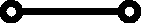
\includegraphics[width=0.15\textwidth]{mt1.pdf}
    \hfill
    2. 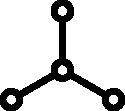
\includegraphics[width=0.15\textwidth]{mt2.pdf}
    \hfill
    3. 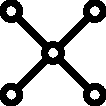
\includegraphics[width=0.13\textwidth]{mt3.pdf}
    \hfill
    4. 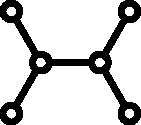
\includegraphics[width=0.15\textwidth]{mt4.pdf}\\
    \bigskip
    5. 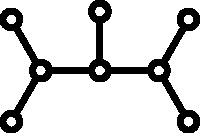
\includegraphics[width=0.23\textwidth]{mt5.pdf}
    \hfill
    6. 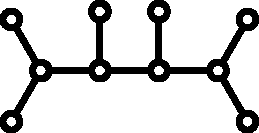
\includegraphics[width=0.3\textwidth]{mt7.pdf}
    \hfill
    7. 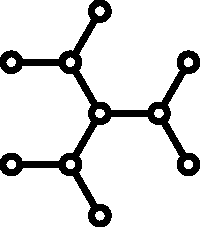
\includegraphics[width=0.22\textwidth]{mt6.pdf}}
    \caption{Семь типов главного дерева}
    \label{fig:7trees}
\end{figure}

% % \begin{figure}[H]
% %     \centering
% %     % \includestandalone[width=0.7\textwidth]{case2}
% %     \caption{Дендриты классов \textbf{(A)}, \textbf{(B)}, \textbf{(C)}, \textbf{(D3)} и \textbf{(D6)}}
% %     \label{img:dentypes}
% % \end{figure}


\begin{proof}
Пусть $K$ --- фрактальный квадрат, являющийся дендритом, с главным деревом $\ga$. 
Все концы этого дерева лежат в $\dd K$.

Пусть $K$ относится к типам {\bf A} или {\bf C}. 
Тогда, по Теореме \ref{ssboundary}, главное $\gamma$ может содержать 2, 3 или 4 конца, что соответствует моделям 1, 2, 3 и 4 на Рисунке \ref{fig:7trees}.


Если $K$ относится к типу {\bf B}, то по Теоремам \ref{ssboundary} и \ref{thm:corner} главное дерево имеет ровно четыре конца, что соответствует моделям 3 и 4.

Если $K$ соответствует типу {\bf D3}, то по Теоремам \ref{ssboundary} и \ref{thm:corner} главное дерево $\gamma$ имеет только 3 конца, что соответствует модели 2.

Если $K$ относится к типу {\bf D6}, то по Теореме \ref{ssboundary} и Лемме \ref{lem:d4bound} главное дерево $\gamma$ может иметь от 2 до 6 концов, и для любого  $x\in \gamma $ верно $ Ord(x,\gamma)\leq3$, поэтому $\gamma$ не может иметь форму, отличную от моделей 1, 2, 4, 5, 6 или 7 с Рисунка \ref{fig:7trees}.
\end{proof}


\begin{remark}
Если $K$ относится к типу {\bf D6}, то его главное дерево $\gamma$ не может иметь форму, отличную от моделей 4, 5, 6 или 7 на рисунке \ref{fig:7trees}.
Невозможность моделей 1 и 2 главного дерева фрактальных квадратов типа {\bf D6} обусловлена тем, что число концов в $\gamma$ для типа {\bf D6} не меньше 4.
Однако для доказательства Теоремы \label{thm:7trees} это не требуется.
\end{remark}

Таким образом, если классифицировать фрактальные квадраты, являющиеся дендритами, по форме главного дерева, то мы получим 7 классов фрактальных квадратов.
Такую классификацию мы можем называть {\em общей классификацией} или {\em классификацией по форме главного дерева}.

Если принять во внимание гипотезу о том, что во фрактальном квадрате типа {\bf D6} число концов в его главном дереве $\gamma$ не меньше 4, то мы можем рассмотреть {\em тонкую классификацию}, учитывающую следующие признаки:
\begin{itemize}[nolistsep]
	\item[1.] форма главного дерева (1 из 7 типов);
	\item[2.] тип самоподобной границы ({\bf A}, {\bf B}, {\bf C}, {\bf D3} или {\bf D6});
	\item[3.] порядки ветвления точек самоподобной границы в главном дереве.
\end{itemize}

Примеры фрактальных квадратов из каждого класса тонкой классификации показаны на следующих рисунках.
Всего получается 16 классов.
Отдельно стоит сказать, что классы 3 ({\bf 2-A-1}) и 4 ({\bf 2-A-2}) с Рисунка \ref{fig:tree2} имеют одинаковый тип дерева и одинаковый тип самоподобной границей, но отличаются порядком ветвления точек самоподобной границы в главном дереве: в {\bf 2-A-1} три конца и одна разбивающая точка, а в {\bf 2-A-2} три конца и одна точка ветвления порядка 3.
Это единственные два класса, которые различаются только по третьему признаку.


\begin{figure}[H]
    \centering
    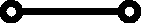
\includegraphics[scale=1.5]{mt1.pdf}
    \vspace{0.5cm}
    \vfill
    \fbox{
    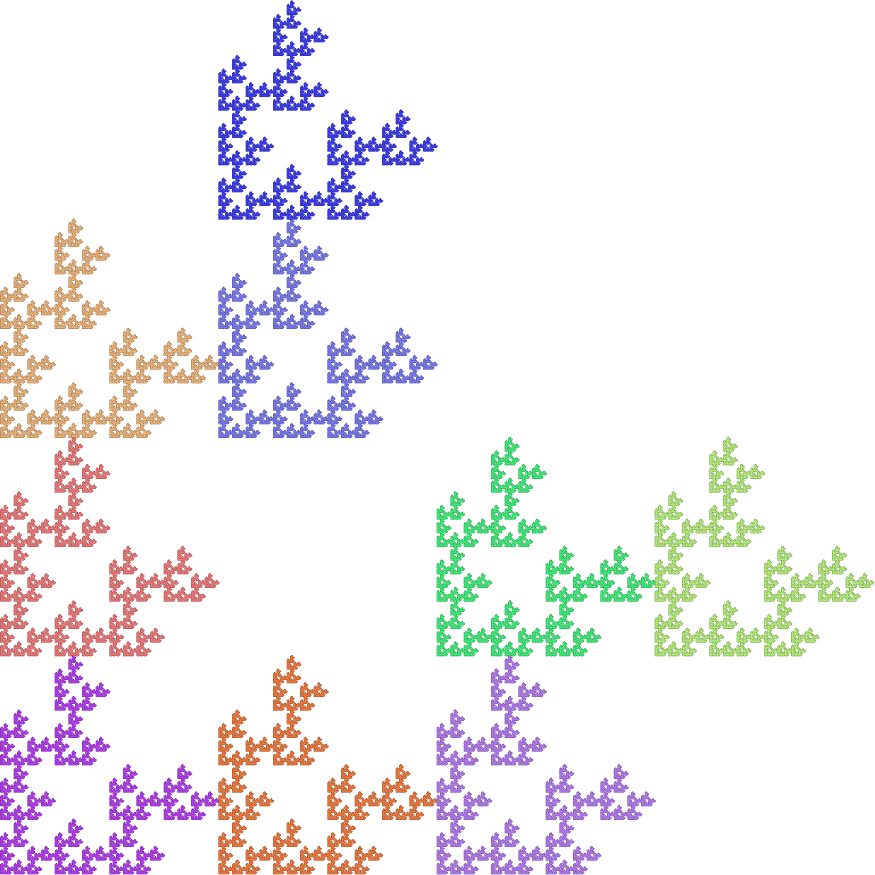
\includegraphics[width=0.22\textwidth]{1K.png}
    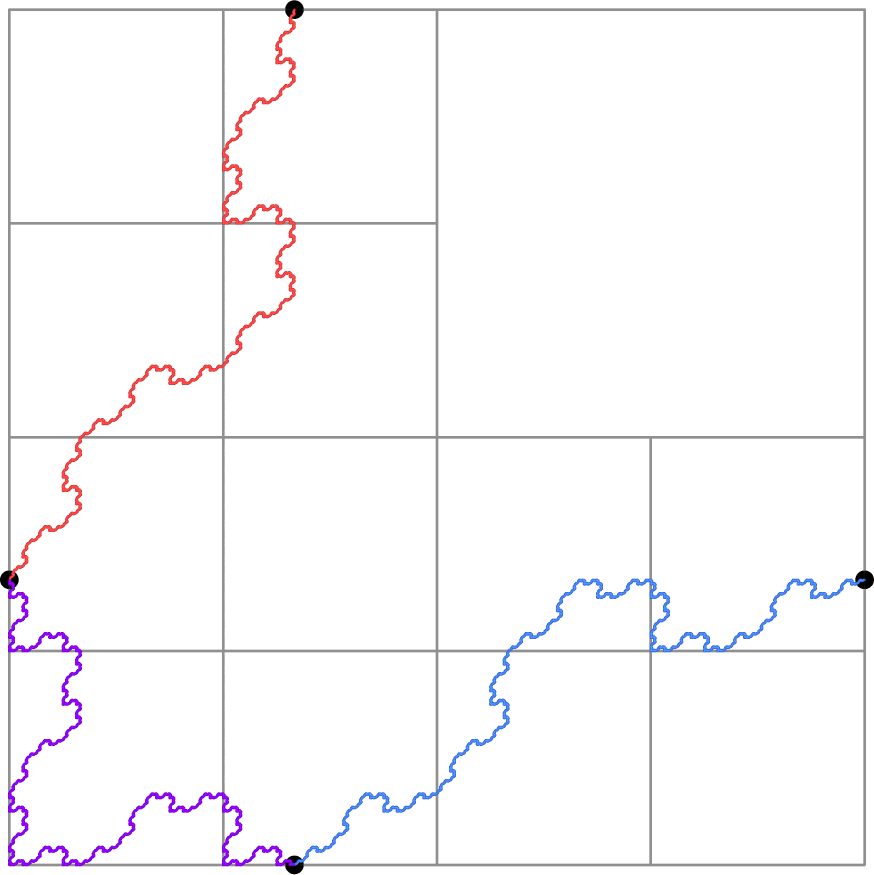
\includegraphics[width=0.22\textwidth]{1T.png}}
    \hfill
    \fbox{
    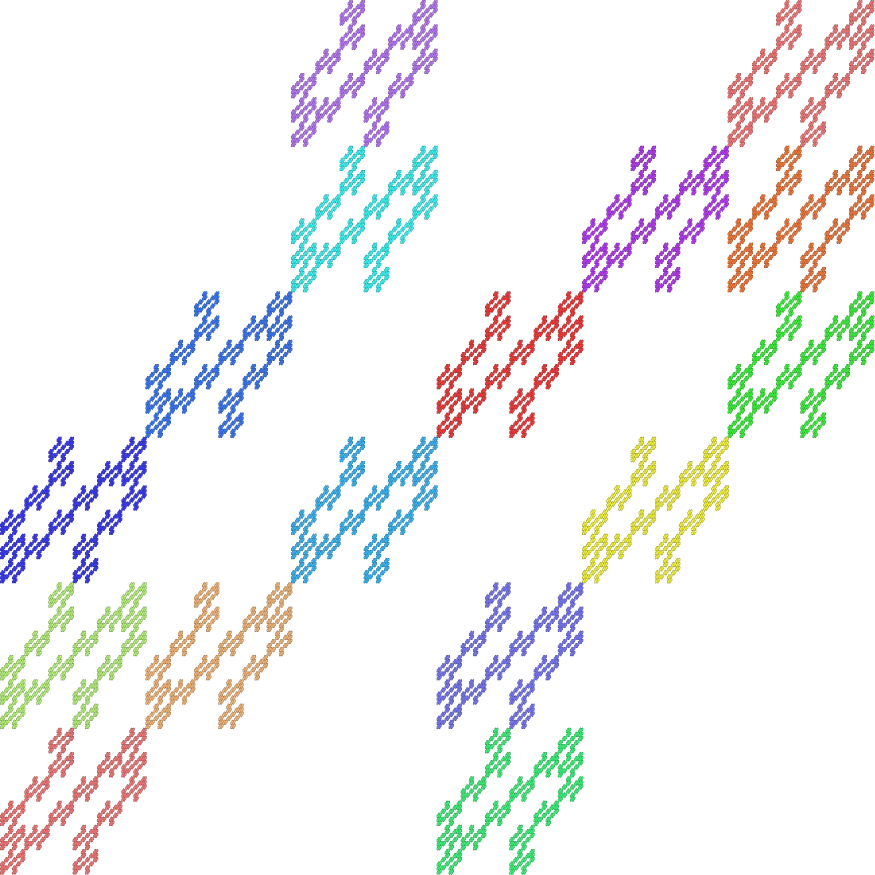
\includegraphics[width=0.22\textwidth]{2K.png}
    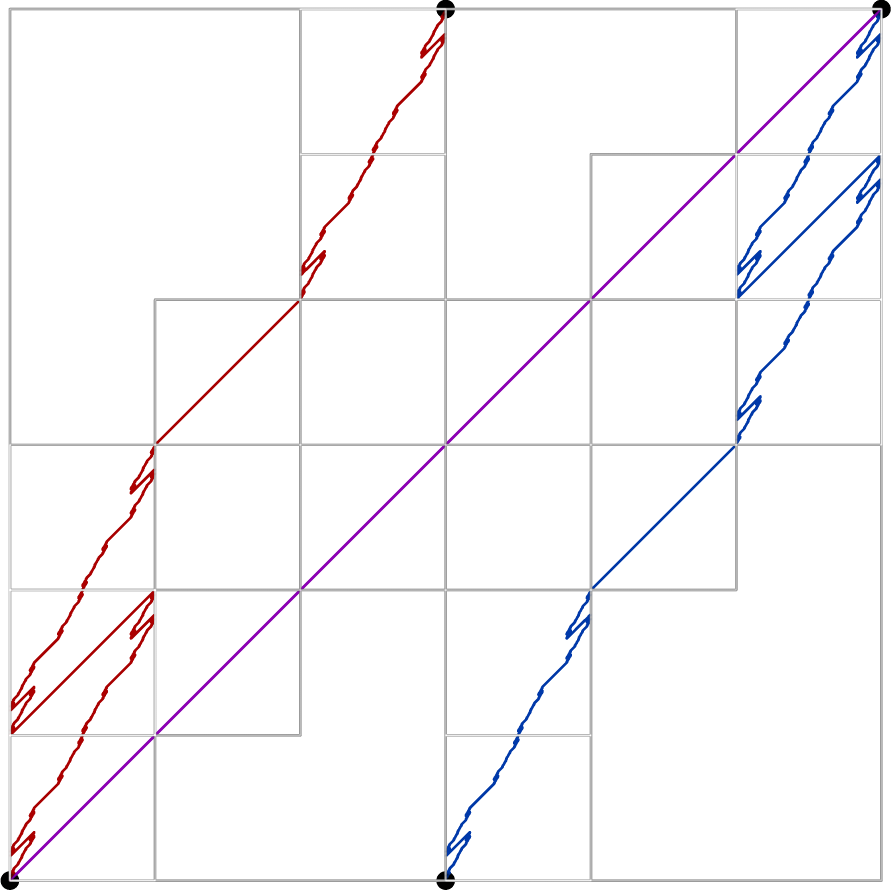
\includegraphics[width=0.22\textwidth]{2T.png}}
    \caption{Дерево 1. Классы 1 и 2 (обозначим как \textbf{1-A} и \textbf{1-C}). }
    \label{fig:tree1}
\end{figure}

\begin{figure}[H]
    \centering
    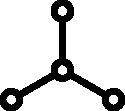
\includegraphics[scale=1.5]{mt2.pdf}
    \vspace{0.5cm}\vfill
    \fbox{
    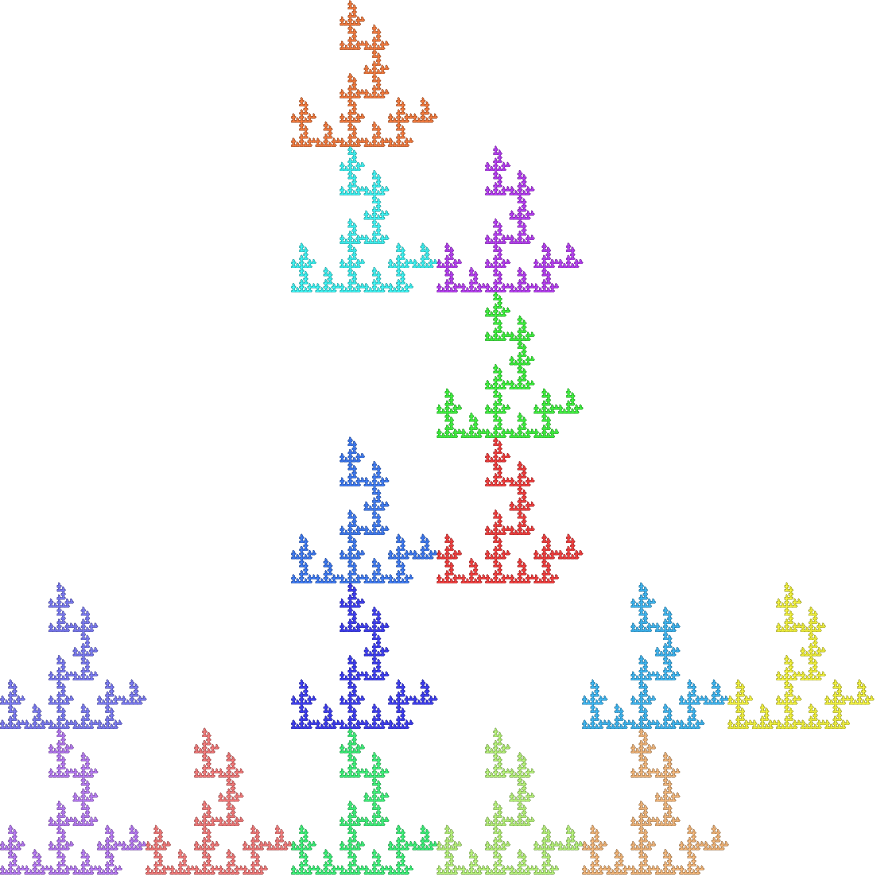
\includegraphics[width=0.22\textwidth]{3K.png}
    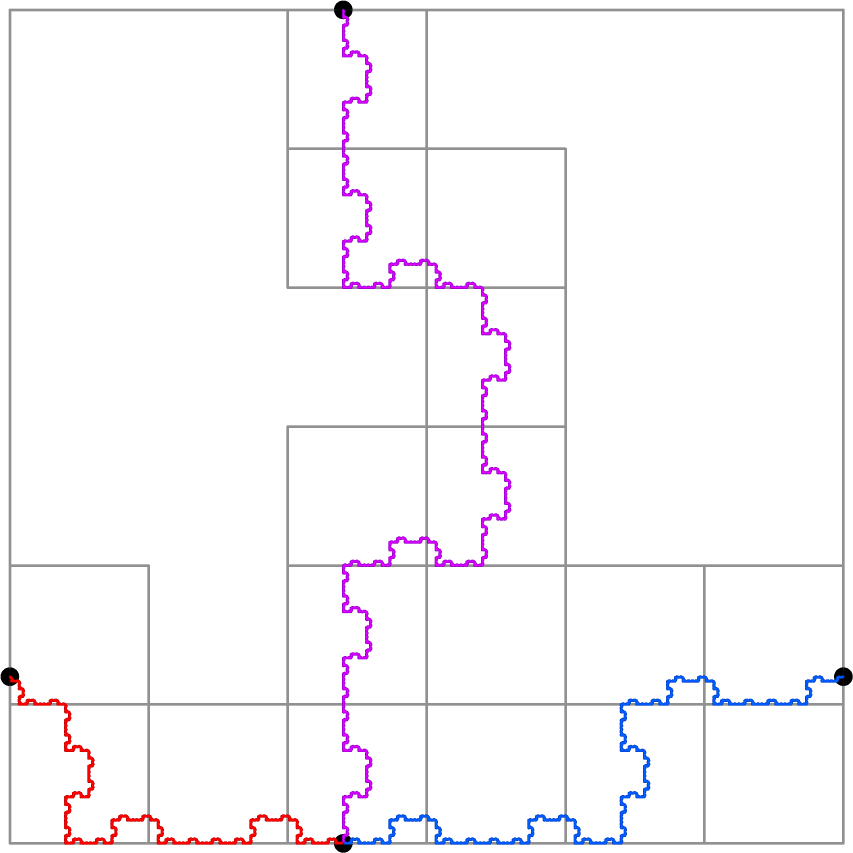
\includegraphics[width=0.22\textwidth]{3T.png}}
    \hfill
    \fbox{
    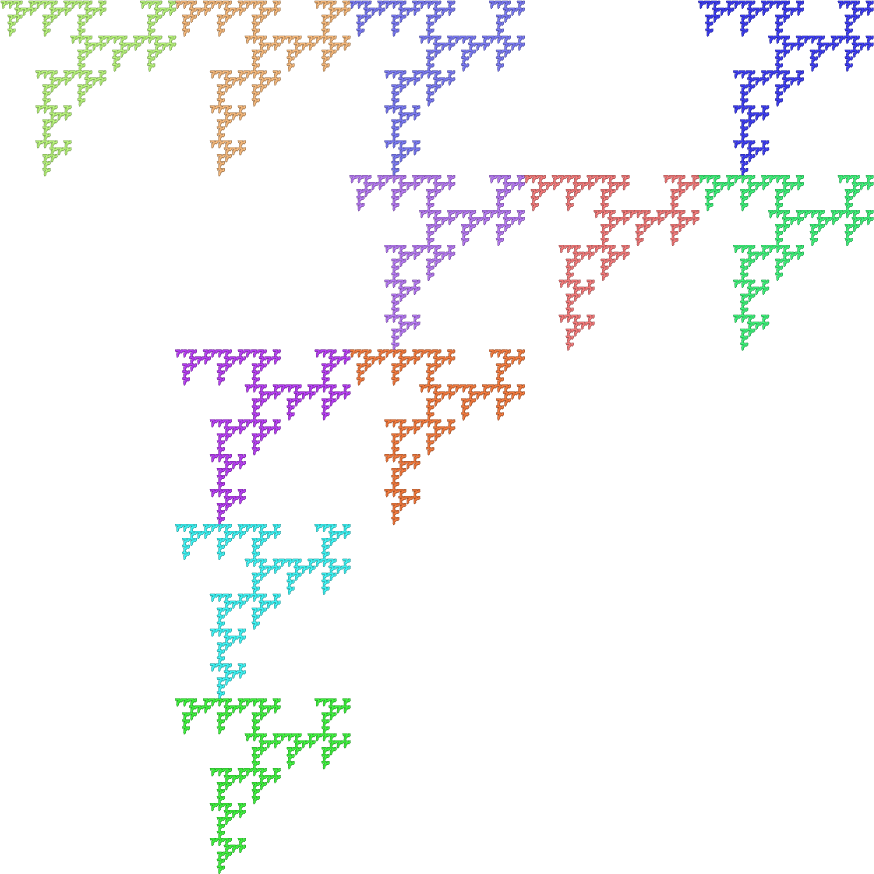
\includegraphics[width=0.22\textwidth]{4K.png}
    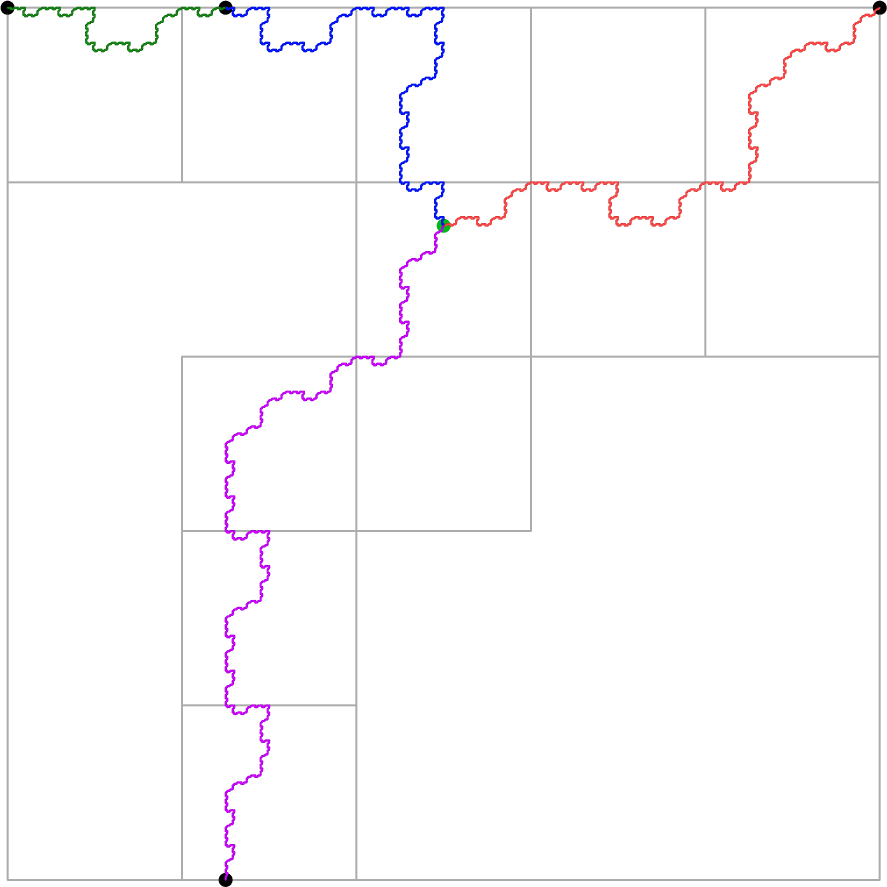
\includegraphics[width=0.22\textwidth]{4T.png}}
    \vspace{0.3cm}\vfill
    \fbox{
    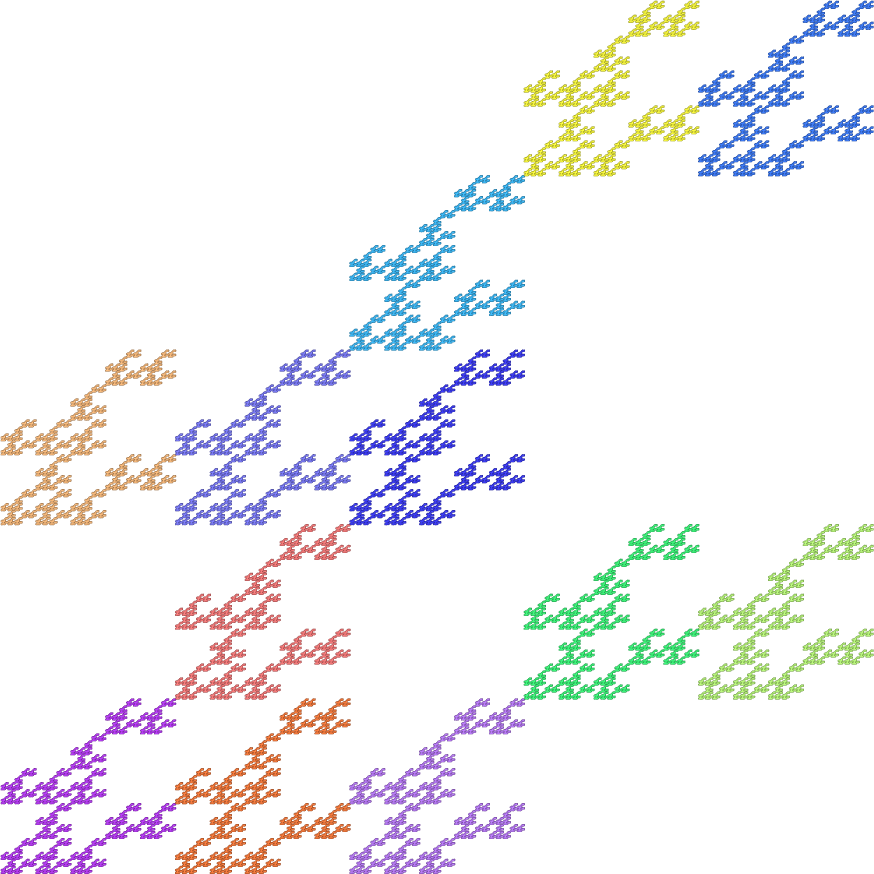
\includegraphics[width=0.22\textwidth]{5K.png}
    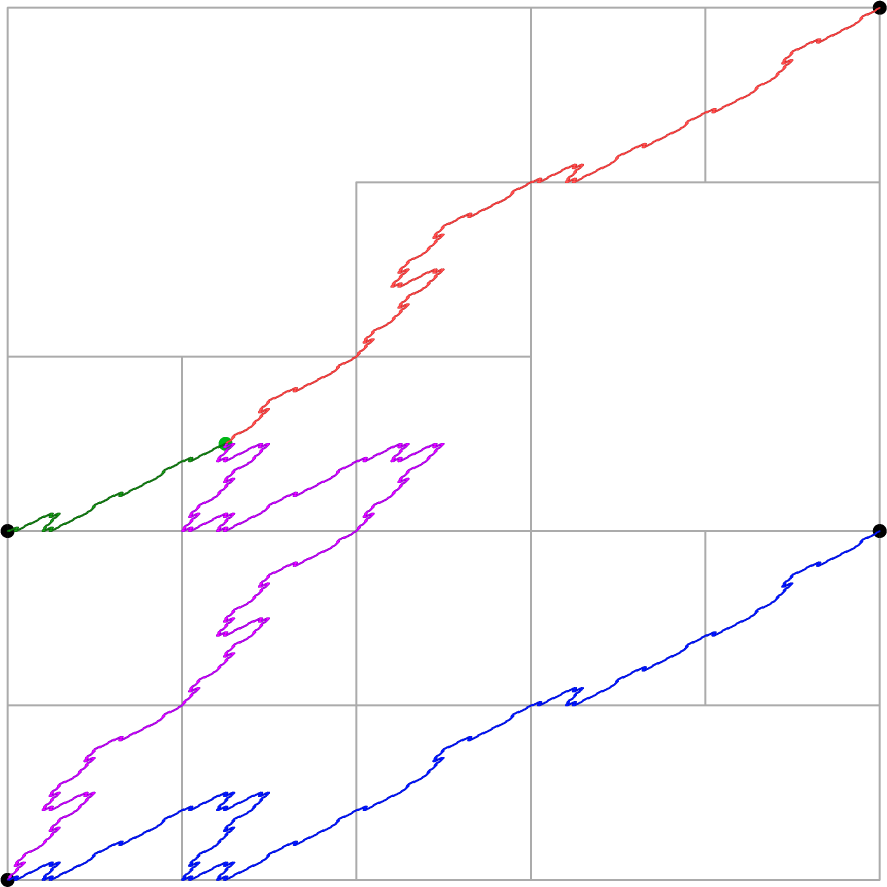
\includegraphics[width=0.22\textwidth]{5T.png}}
    \hfill
    \fbox{
    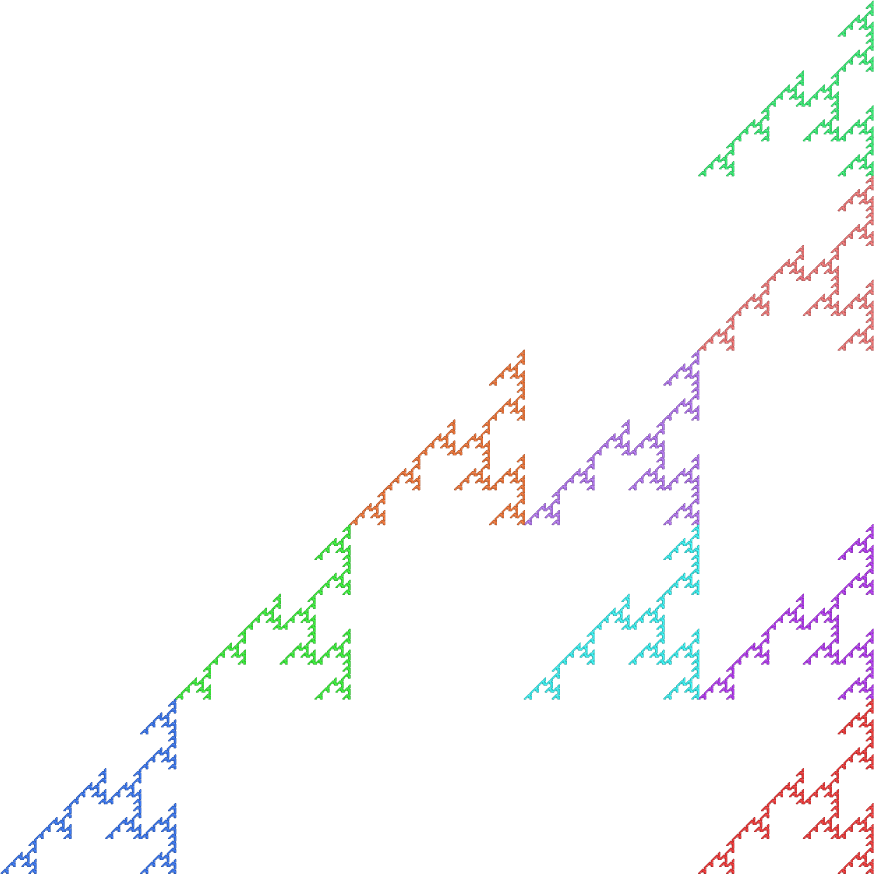
\includegraphics[width=0.22\textwidth]{6K.png}
    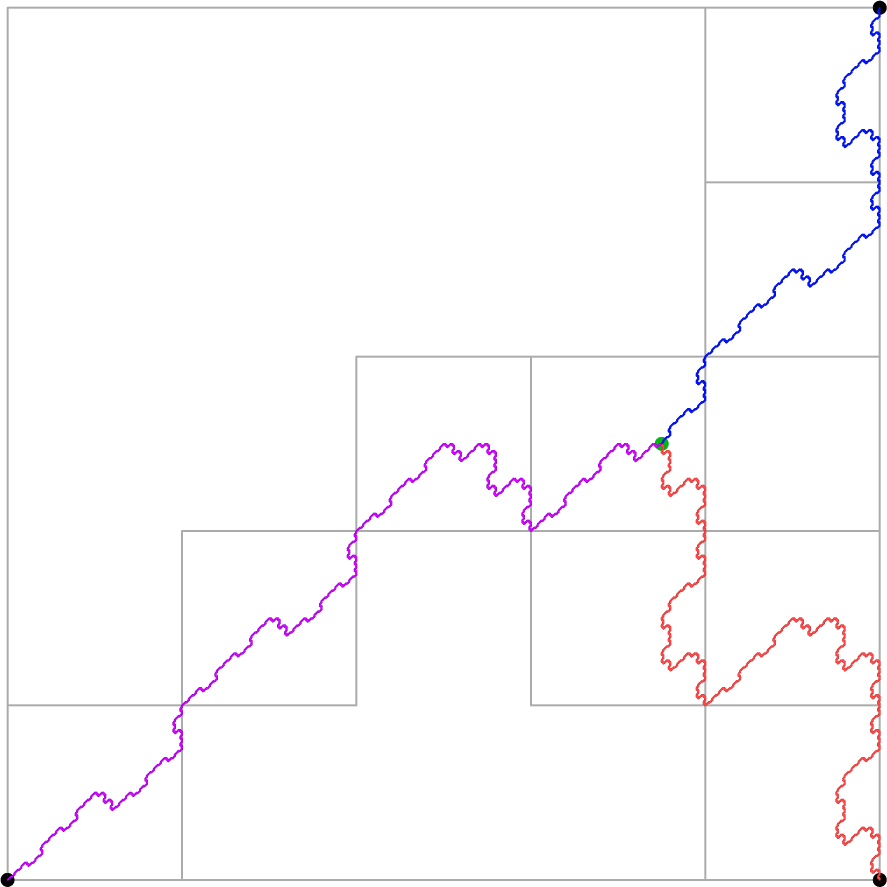
\includegraphics[width=0.22\textwidth]{6T.png}}
    \caption{Дерево 2. Классы 3 ({\bf 2-A-1}), 4 ({\bf 2-A-2}), 5 ({\bf 2-D6}) и 6 ({\bf 2-D3})}
    \label{fig:tree2}
\end{figure}

\begin{figure}[H]
    \centering
    \hspace{0.12\textwidth}
    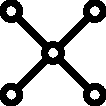
\includegraphics[scale=1.5]{mt3.pdf}
    \hfill
    \fbox{
    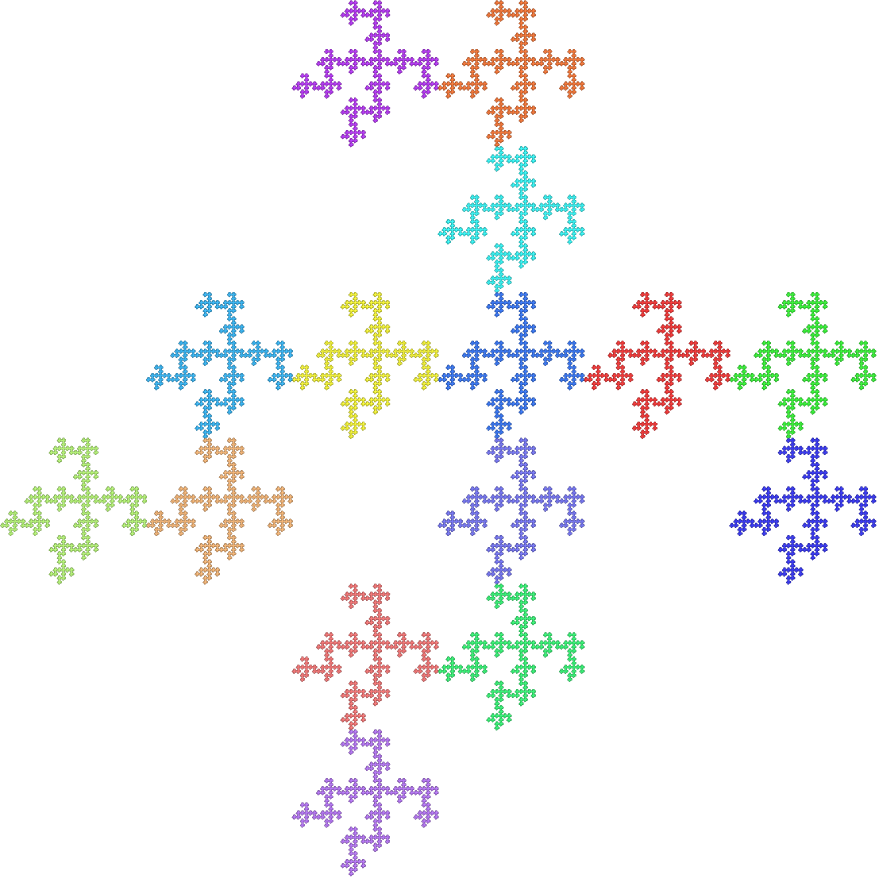
\includegraphics[width=0.22\textwidth]{7K.png}
    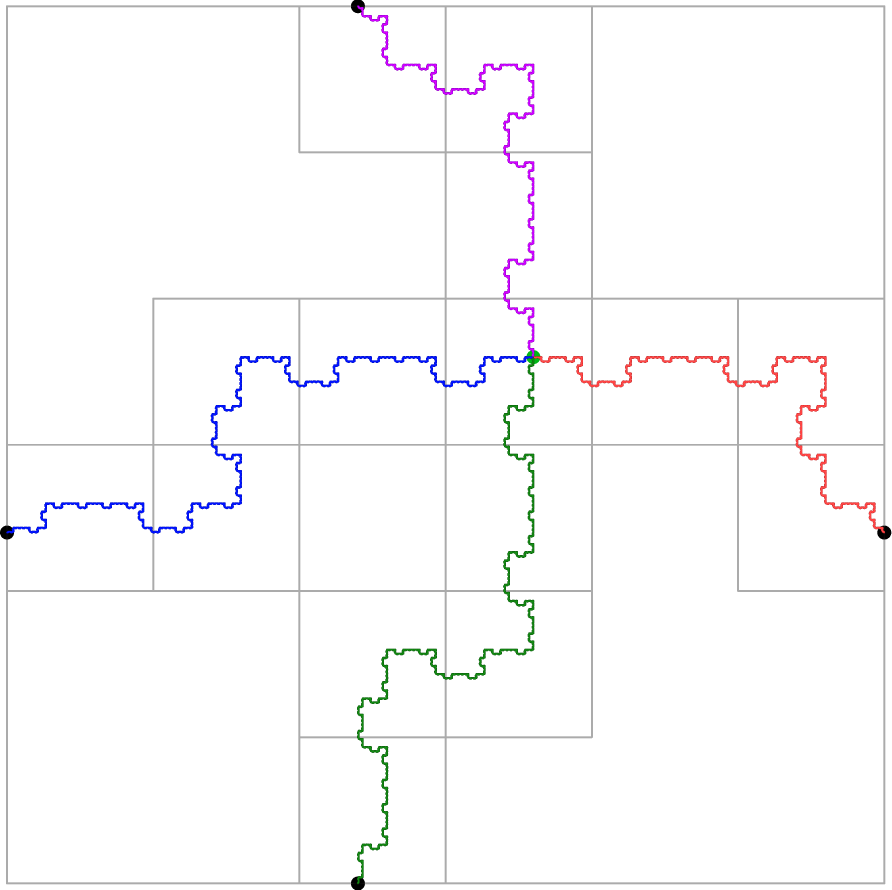
\includegraphics[width=0.22\textwidth]{7T.png}}
    \vspace{0.3cm}\vfill
    \fbox{
    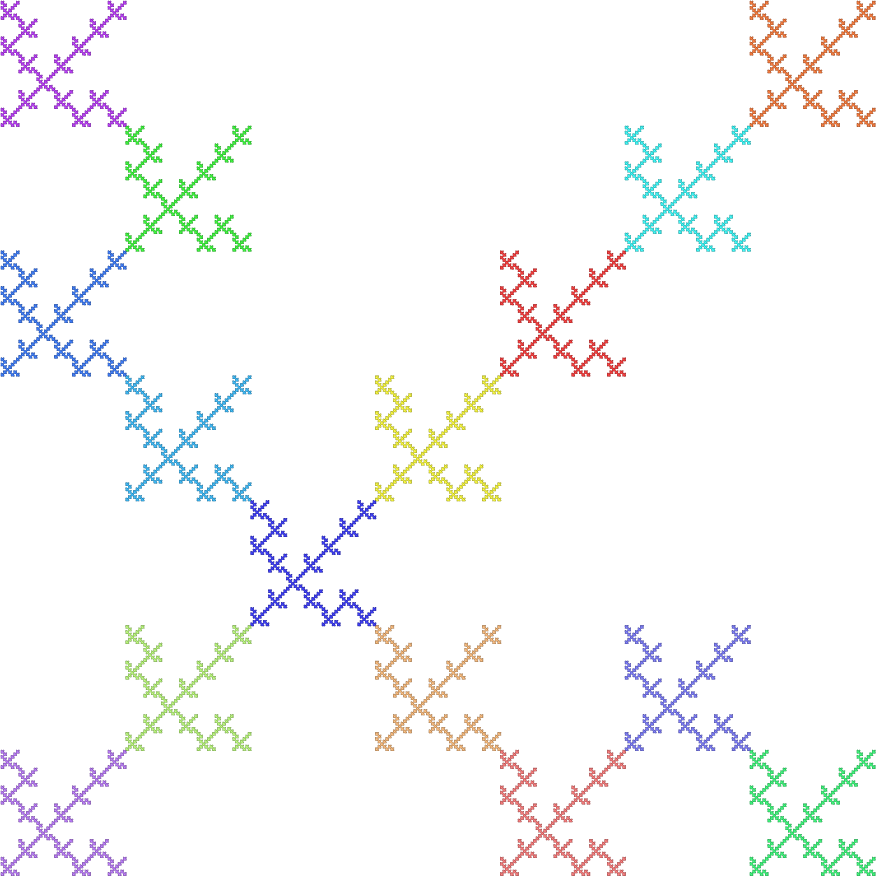
\includegraphics[width=0.22\textwidth]{8K.png}
    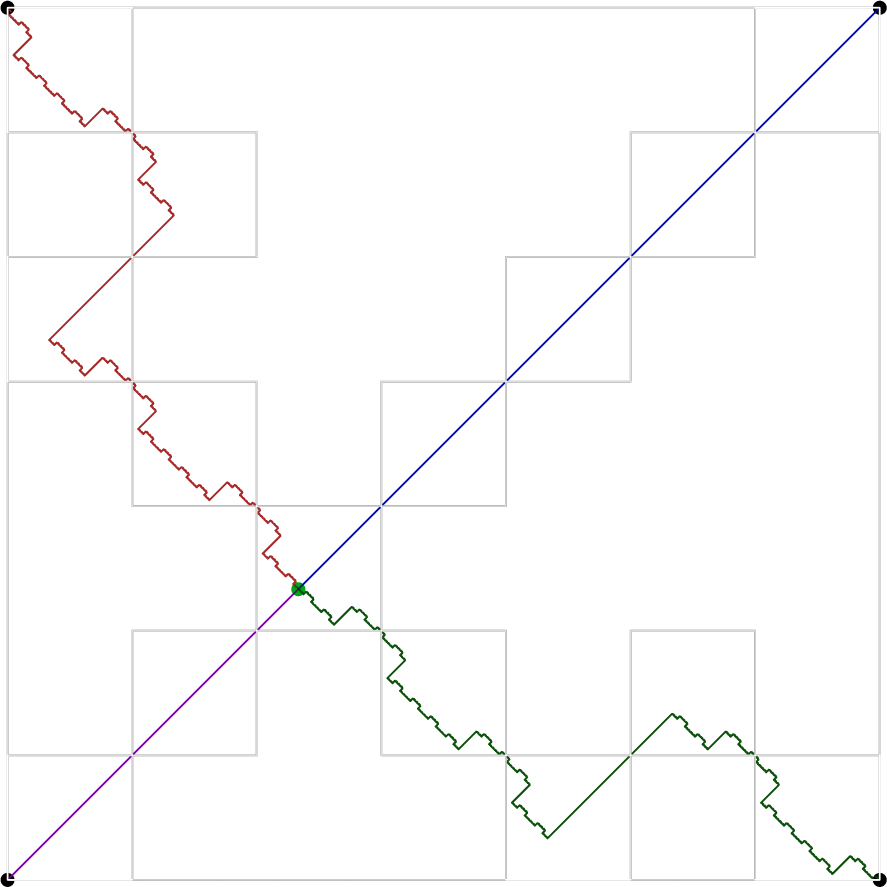
\includegraphics[width=0.22\textwidth]{8T.png}}
    \hfill
    \fbox{
    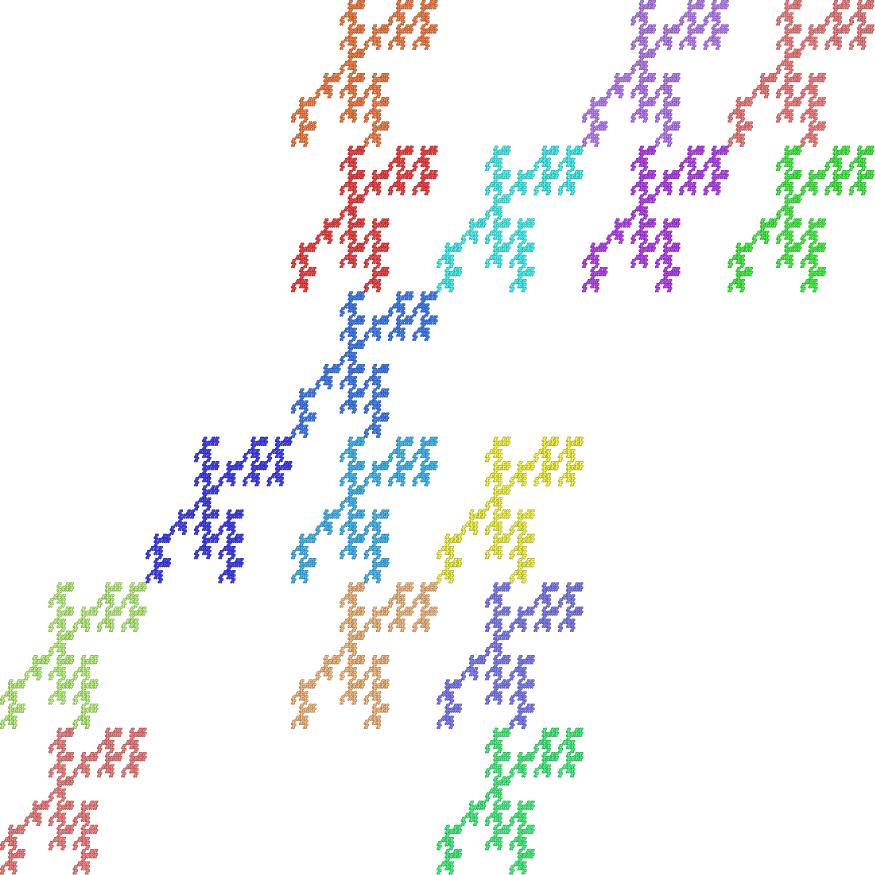
\includegraphics[width=0.22\textwidth]{9K.png}
    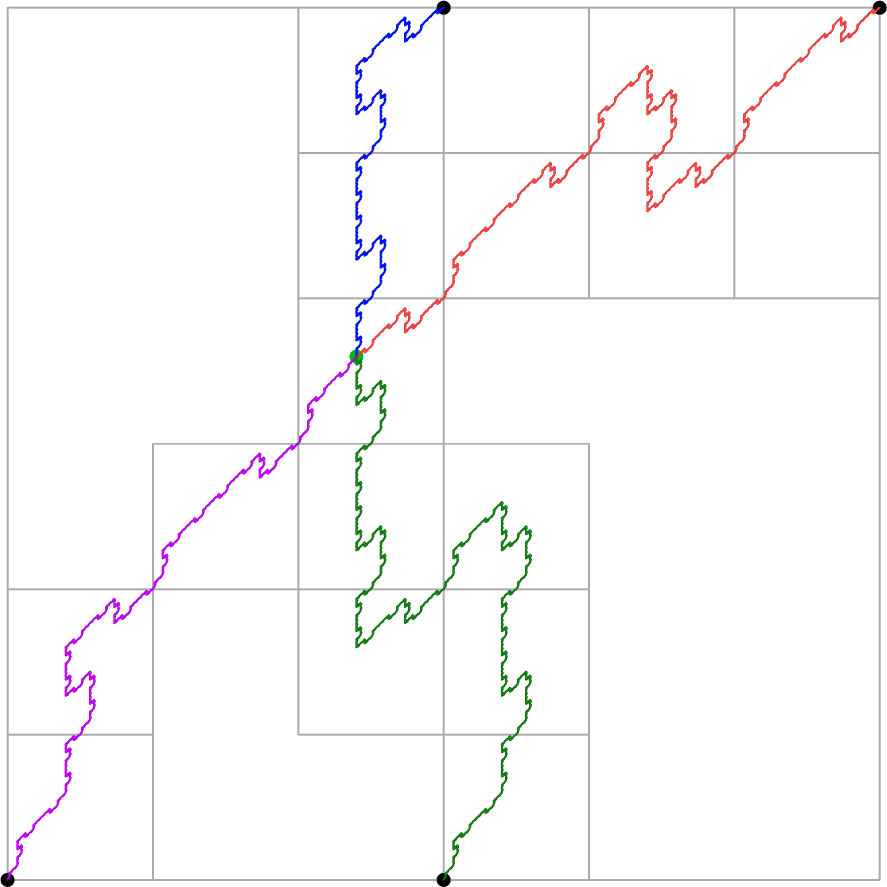
\includegraphics[width=0.22\textwidth]{9T.png}}
    \caption{Дерево 3. Класс 7 ({\bf 3-A}), 8 ({\bf 3-B}) и 9({\bf 3-C})}
    \label{fig:tree3}
\end{figure}
 
\begin{figure}[H]
    \centering
    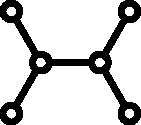
\includegraphics[scale=1.5]{mt4.pdf}
    \vspace{0.5cm}\vfill
    \fbox{
    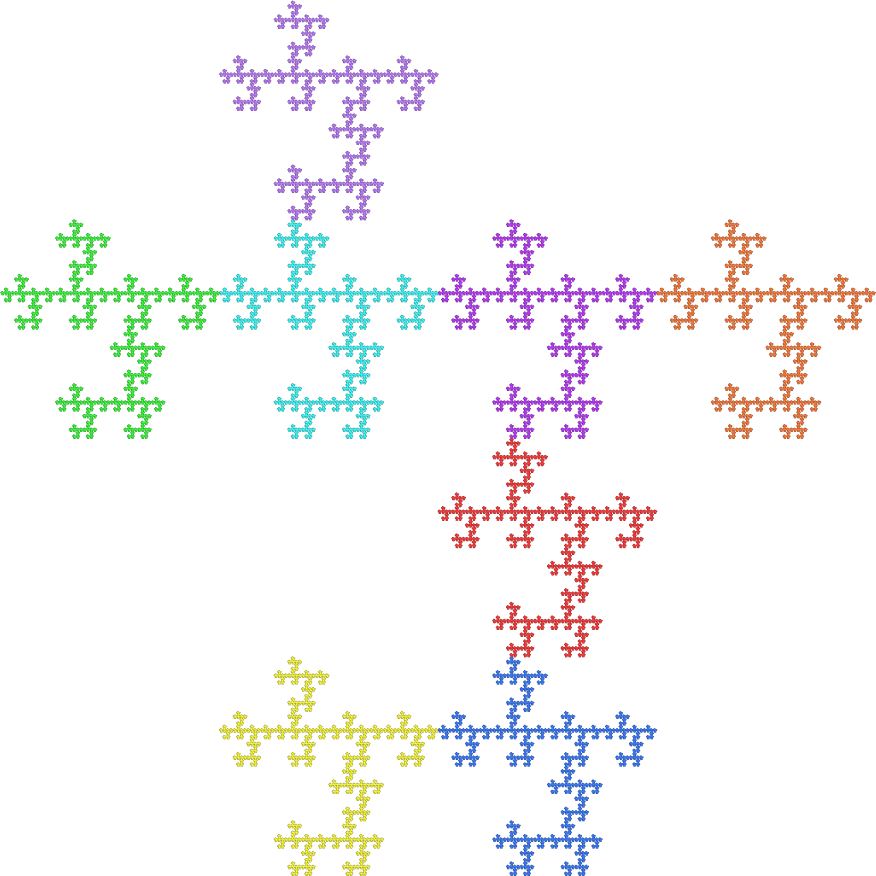
\includegraphics[width=0.22\textwidth]{10K.png}
    \includegraphics[width=0.22\textwidth]{10T.png}}
    \hfill
    \fbox{
    \includegraphics[width=0.22\textwidth]{11K.png}
    \includegraphics[width=0.22\textwidth]{11T.png}}
    \vspace{0.3cm}\vfill
    \fbox{
    \includegraphics[width=0.22\textwidth]{12K.png}
    \includegraphics[width=0.22\textwidth]{12T.png}}
    \hfill
    \fbox{
    \includegraphics[width=0.22\textwidth]{13K.png}
    \includegraphics[width=0.22\textwidth]{13T.png}}
    \caption{Дерево 4. Классы 10 ({\bf 4-A}), 11 ({\bf 4-B}), 12 ({\bf 4-C}) и 13 ({\bf 4-D6})}
    \label{fig:tree4}
\end{figure}

\begin{figure}[H]
    \centering
    \includegraphics[scale=1.4]{mt5.pdf}
    \hfill
    \fbox{
    \includegraphics[width=0.22\textwidth]{14K.png}
    \includegraphics[width=0.22\textwidth]{14T.png}}
    \caption{Дерево 5. Класс 14 ({\bf 5-D6})}
    \label{fig:tree5}
\end{figure}

\begin{figure}[H]
    \centering
    \includegraphics[scale=1.4]{mt7.pdf}
    \hfill
    \fbox{
    \includegraphics[width=0.22\textwidth]{15K.png}
    \includegraphics[width=0.22\textwidth]{15T.png}}
    \caption{Дерево 6. Класс 15 ({\bf 6-D6})}
    \label{fig:tree6}
\end{figure}

\begin{figure}[H]
    \centering
    \includegraphics[scale=1.2]{mt6.pdf}
    \hfill
    \fbox{
    \includegraphics[width=0.22\textwidth]{16K.png}
    \includegraphics[width=0.22\textwidth]{16T.png}}
    \caption{Дерево 7. Класс 16 ({\bf 7-D6})}
    \label{fig:tree7}
\end{figure}
